%%%%%%%%%%%%%%%%%%%%%%%%%%%%%%%%%%%%%%%%%%%%%%%%%%%%%%%%%%%%%%%
\section{Photon Detection System Design}
\label{sec:fdsp-pd-design}
%\metainfo{(Length: \dword{tdr}=50 pages, TP=20 pages)}
%\metainfo{\color{blue} Content: Conveners}

%dww edits 16mar18
%rjw edits 15-17mar18

The principal task of the \dword{spmod}\dword{pds} is to measure the \dword{vuv} scintillation light produced by ionizing tracks in the TPC within the geometrical constraints of the \dword{apa} structure. A commercially available compact solution for photon measurement is the \dword{sipm}, however, the response of the devices, which typically peaks in the visible range (>\SI{400}{nm}) is not well-matched to incident \SI{127}{nm} scintillation photons, so a wavelength shifter or some sort must be employed. 
In addition, even though production cost and key performance parameters have improved significantly in recent years, the cost of the readout electronics (channel count) and the \dword{sipm}s needed to meet the physics requirements of the \dword{pds} would be prohibitive. 

The photon collector must optimize the costs of various components of the system while meeting the performance requirements.  In practice, this consists of collecting \dword{vuv} photons over an area of hundreds of square-meters (viewing the entire \SI{10}{kt} \lar fiducial mass), converting the photons to longer wavelengths and guiding them onto \dwords{sipm} that are typically O(cm$^2$). For reference, an array of \num{48} \dwords{sipm}
\footnote{Twelve 4x4 arrays of \SI{3}{mm}$\times$\SI{3}{mm} sensL C-series coated with \SI{100}{$\mu$g/cm$^2$} of \dword{tpb}, tested in the Fermilab \dword{tallbo} \lar facility with an alpha source (Am241).}  
demonstrated a detection efficiency of 13\%, corresponding to an effective area of \SI{2.2}{cm$^2$}.
%\footnote{An array of 12 SensL 4x4 arrays of \SI{3}{mm}$\times$\SI{3}{mm} SensL C-series \dwords{sipm} (48 in all)  coated with \dword{tpb} and mounted on an active ganging board. This detector tested in the Fermilab \dword{tallbo} \lar facility with an alpha source (Am241) in March 2017. With a coating of \SI{100}{$\mu$g/cm$^2$} of \dword{tpb} the array demonstrated an efficiency of 13\%.}. 


A challenge for the \dword{pds} is that a full set of requirements is not yet fully defined for one of the priority physics topics, \dword{snb} neutrinos. So the designs strive to demonstrate that at minimum the requirements for the accelerator neutrino program, atmospheric neutrinos and nucleon decay will be met, while maintaining the flexibility to adjust to the greater demands for the SBN physics.    
 
%The core modular element of the \dword{pds} are the large area \textit{photon collectors} that convert incident \SI{128}{nm} scintillation photons into photons in the visible range (>~\SI{400}{nm}), which in turn are converted to an electrical signal by compact silicon photomultipliers (\dword{sipm}) \textit{photon sensors}.  At the time of the Technical Proposal there are three photon collector options under consideration; Figure~\ref{fig:3dtpc-pd} shows how they are incorporated into the TPC anode plane assembly by an identical modular mounting scheme. In the following we summarize the design and development status for each photon collector option\footnote{For the \dword{tdr} there will be a baseline design and at most one alternative.}.

At the time of the Technical Proposal there are three photon collector options under consideration; Figure~\ref{fig:3dtpc-pd} shows how they are incorporated into the TPC anode plane assembly by an identical modular mounting scheme. In the following we summarize the design and development status for each photon collector option\footnote{For the \dword{tdr} there will be a baseline design and at most one alternative.}.

%%%%%%%%%%%%%%%%%%%%%%%%%%%%%%%%%%%
%\subsection{Photon Collector}
%\label{sec:fdsp-pd-pc}
%\metainfo{\color{blue} Content: Cavanna/Whittington/Machado}


\subsection{Photon Collector: ARAPUCA}
\label{ssec:fdsp-pd-pc-arapuca}
%\todo{\color{blue} Content: A.Machado}

The ARAPUCA is a device based on a new approach to \lar scintillation photon detection where the effective photon detection area is increased by trapping photons inside a box with highly reflective internal surfaces until reflections guide them to a much smaller \dword{sipm}~\cite{arapuca_jinst}. 

Photon trapping is achieved through a novel use of wavelength-shifting and the technology of the dichroic shortpass optical filters. These commercially available filters are created by using multilayer thin films that in combination have the property of being highly transparent to photons with a wavelength below a tunable cut-off while being almost perfectly reflective to photons with wavelength above the cut-off.  Such a filter coated with either one or two different wavelength-shifters, depending on the detailed implementation,  forms the entrance window to a flat box with internal surfaces covered by highly reflective acrylic foils
%(3M-Vikuiti ESR \footnote{3M Vikuiti\texttrademark\ ~foils. https://en.wikipedia.org/wiki/Vikuiti.}, for example), 
except for a small fraction of the surface that is occupied by active photosensors (\dwords{sipm}).

To act as a photon trap, the wavelength-shifter deposited on the outer face of the dichroic filter must have its emission wavelength \textit{less} than the cut-off wavelength of the filter, below which transmission is typically greater than 95\%. These photons pass through the filter where they encounter a second wavelength-shifter, either on the inner surface of the filter or coated on the reflecting inner surfaces of the box,
with an emission spectrum greater than the cut-off wavelength. For these photons the reflectivity of the filter is typically greater than 98\%, so they will reflect off the filter surface (and the inner walls) and so be trapped inside the box with a high probability to be incident on an \dword{sipm} before being lost to absorption. The concept is illustrated in Figure \ref{fig:arapuca}, in this example the filter cut-off is \SI{400}{nm}.

%In a \lar volume, a fraction of the scintillation \dword{vuv} photons ($\lambda \sim$ \SI{127}{nm}) produced by the passage of an ionizing radiation, hit the window of the ARAPUCA and are shifted to a wavelength of L$_1$ by the shifter deposited on the external face of the filter and a significant fraction travel towards the internal cavity of the ARAPUCA. On the coated surface inside the box the photons are converted to the wavelength L$_2$ and so are effectively trapped inside the box since the internal surface of the box is covered with a very high reflectance material in this wavelength range and the filter that forms the one-way window into  the box is itself reflective to L$_2$ photons.  After a few reflections the photons are detected by the \dword{sipm} installed on the internal surface of the ARAPUCA (Figure \ref{arapuca}). 

The net effect of the ARAPUCA is to amplify the active area of the \dword{sipm} used to readout the trapped photons. It is easy to show that, for small values of \dword{sipm} coverage of the internal surface, the amplification factor is equal to $A=1/(2(1-R))$,
%\begin{equation}
%A=\frac{1}{2(1-R)}
%\end{equation}
where R is the average value of the reflectivity of the internal surfaces; for an average reflectivity of 0.95 the amplification factor is equal to ten.

\begin{dunefigure}[Schematic representation of the ARAPUCA operating principle.]{fig:arapuca}
{Schematic representation of the ARAPUCA operating principle.}
%  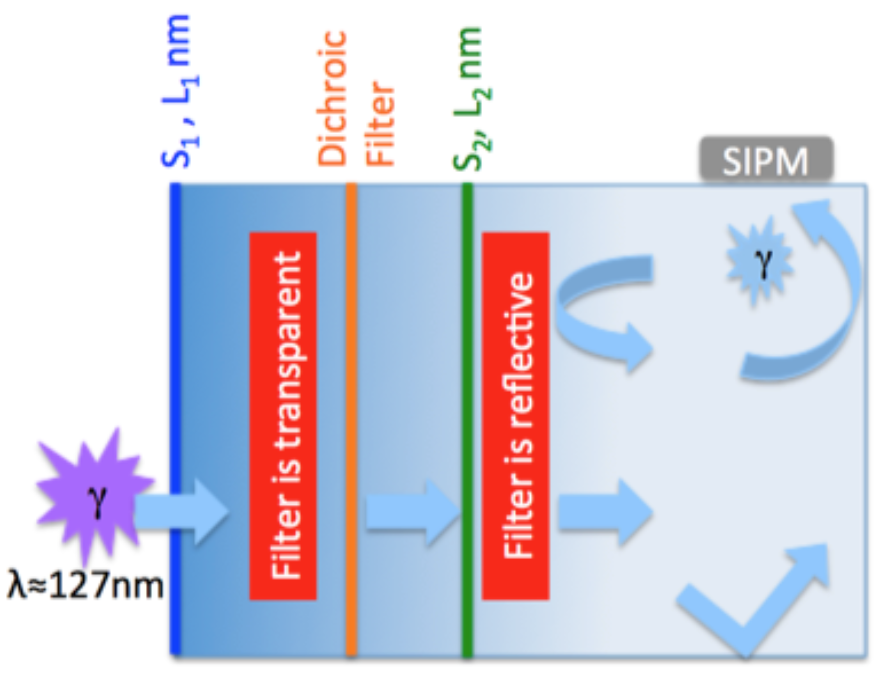
\includegraphics[height=5cm]{pds-arpkscheme}   
  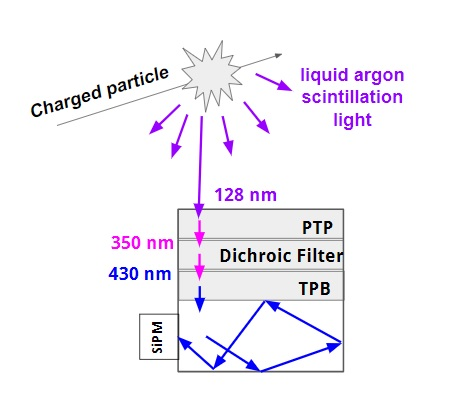
\includegraphics[height=7cm]{pds-arapuca-concept}   
\end{dunefigure}


\subsubsection{Prototype Measurements}
%\subsubsection{Measurements performed in Brazil}
\label{subsec:testlnls}

ARAPUCA prototypes with different configurations have been tested in \lar at multiple facilities. In each case, the first wavelength shift of \SI{127}{nm} scintillation photons down to \SI{350}{nm} that can pass through the filter substrate was performed by p-TerPhenyl (pTP) evaporated onto the outside of a dichroic filter window. 

The first prototype was made of PTFE with internal dimensions of \SI{3.5}{cm}$\times$\SI{2.5}{cm}$\times$\SI{0.6}{cm} with a window formed from a dichroic filter with dimensions of \SI{3.5}{cm}$\times$\SI{2.5}{cm} and wavelength cut-off at \SI{400}{nm}. 
TetraPhenyl-Butadiene (\dword{tpb}) was evaporated onto the internal side of the filter where it absorbs the shifted \SI{350}{nm} photons and reemits around \SI{430}{nm}. Trapped light is detected by a single \SI{0.6}{cm}$\times$\SI{0.6}{cm} sensL \dword{sipm} mod C60035\footnote{http://sensl.com/products/c-series/}.
The device was installed inside a vacuum tight stainless-steel cylinder closed by two CF100 flanges. The cylinder was deployed inside a \lar open bath, vacuum pumped down to a pressure around  10$^{-6}$~\si{mbar} and then filled with one liter of ultra-pure \lar\footnote{Argon 6.0, less than \SI{1}{ppm} total residual contamination.}.

Scintillation light emission was produced by an alpha source\footnote{A $^{238}$U-Al alloy in the form of a metallic foil, with alpha particle emission of 4.267 MeV.} installed in front of the ARAPUCA immersed in \lar. Signals were read out through an Aquiris\footnote{Aquiris High-Speed Digitizer products; http://www.acqiris.com/.} PCI board and stored on a computer.
%Figure \ref{LNLS_test} shows ARAPUCA and the cryogenic system on the Toroidal Grating Monochromator (TGM) beamline at the Brazilian Synchrotron Light Laboratory (LNLS). 
Figure \ref{LNLS_test} shows photographs of the ARAPUCA and cryogenic system 
%in the Toroidal Grating Monochromator (TGM)  beamline of 
at the Brazilian Synchrotron Light Laboratory (LNLS). 

\begin{dunefigure}[ARAPUCA test at the Brazilian Synchrotron Light Laboratory.]{LNLS_test}
{ARAPUCA test at the Brazilian Synchrotron Light Laboratory} 
	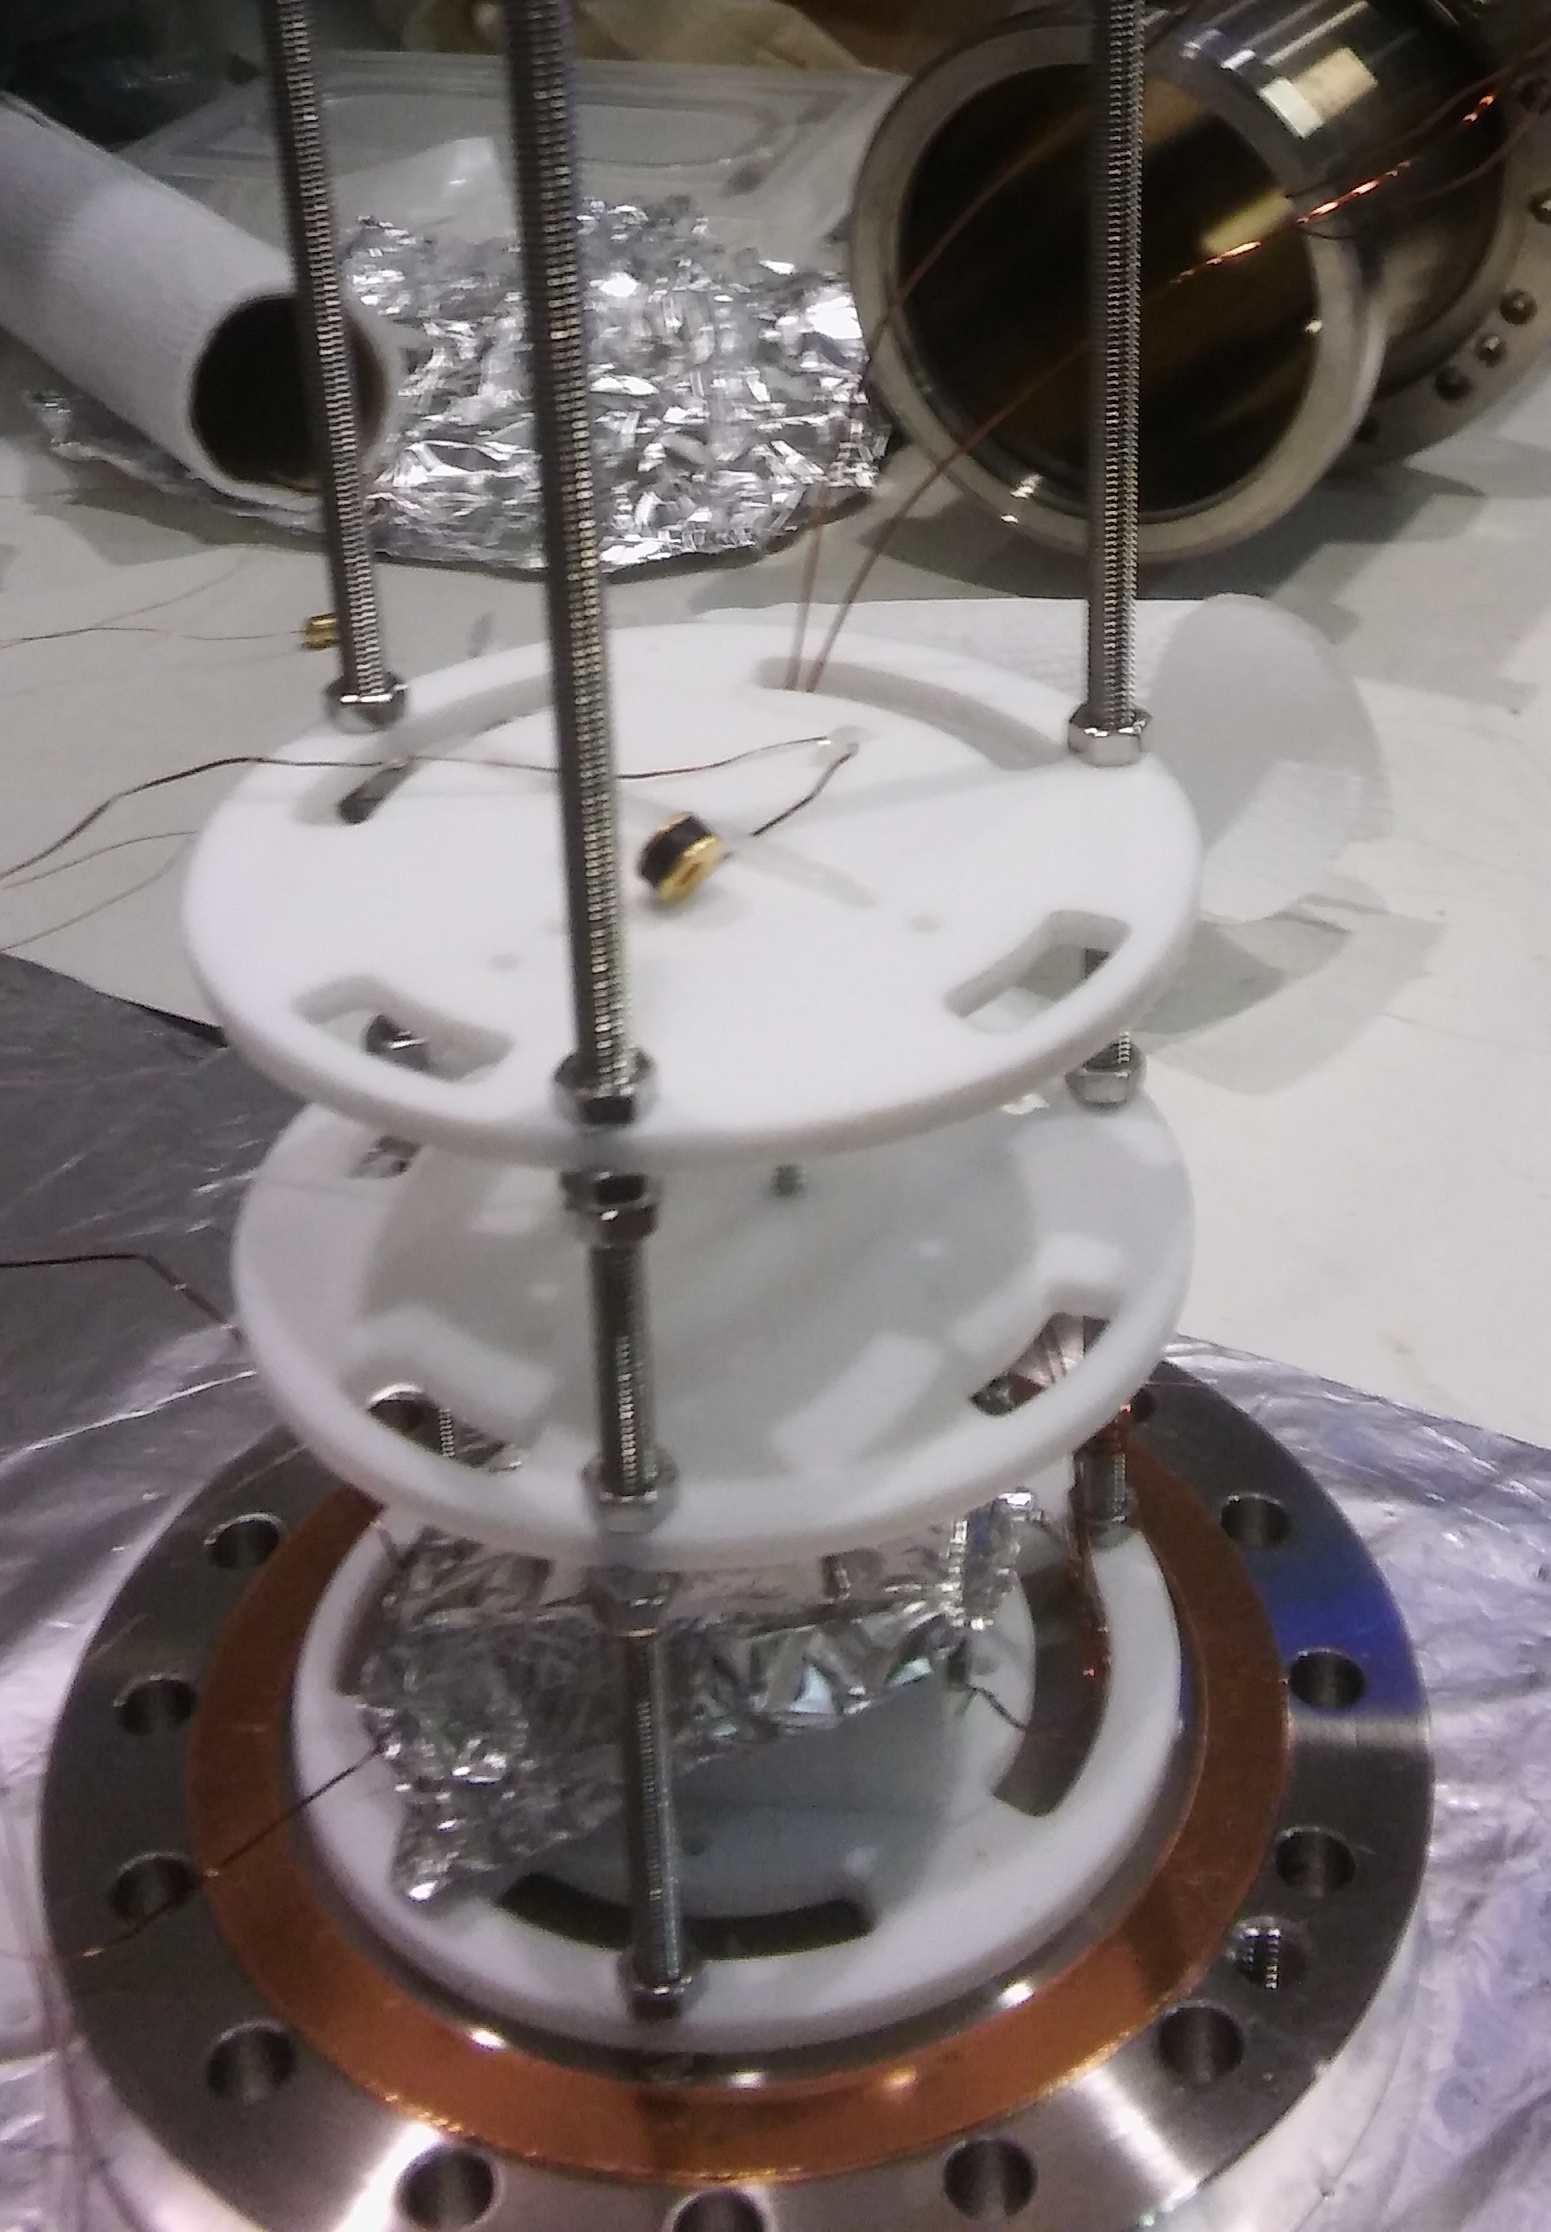
\includegraphics[height=6cm]{pds-tgm_1} \quad
	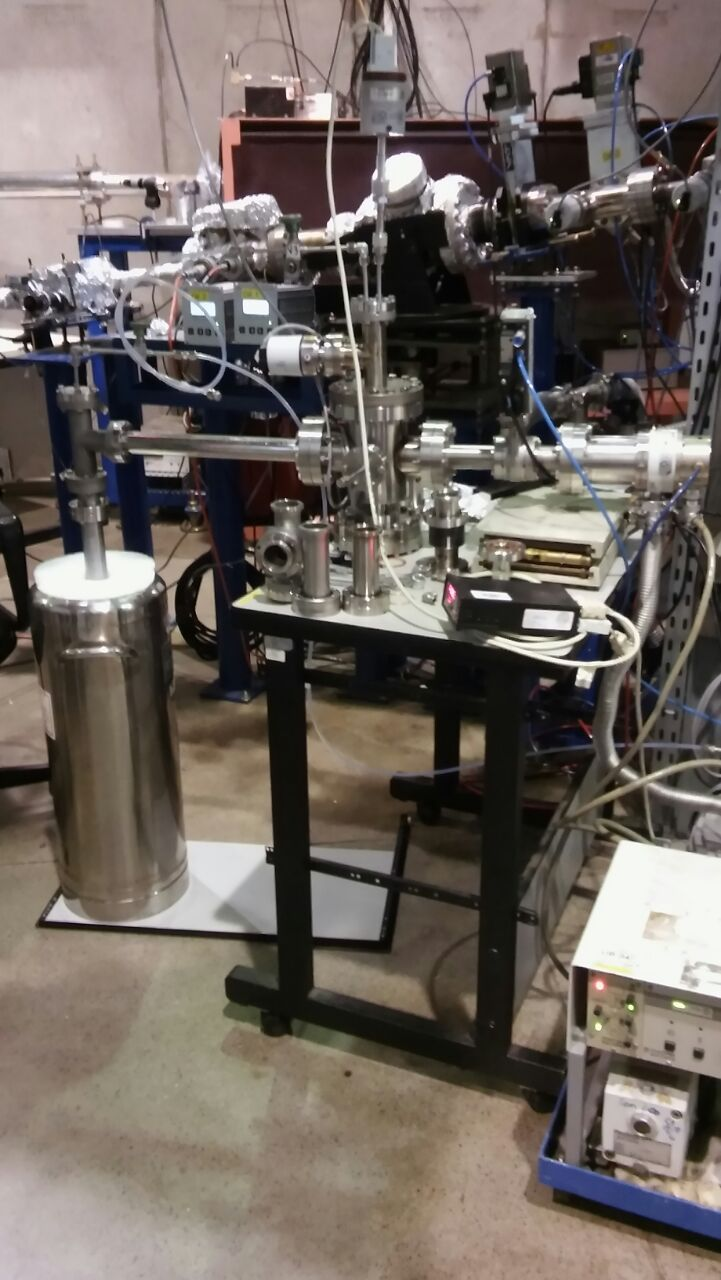
\includegraphics[height=6cm]{pds-tgm_30}\quad
	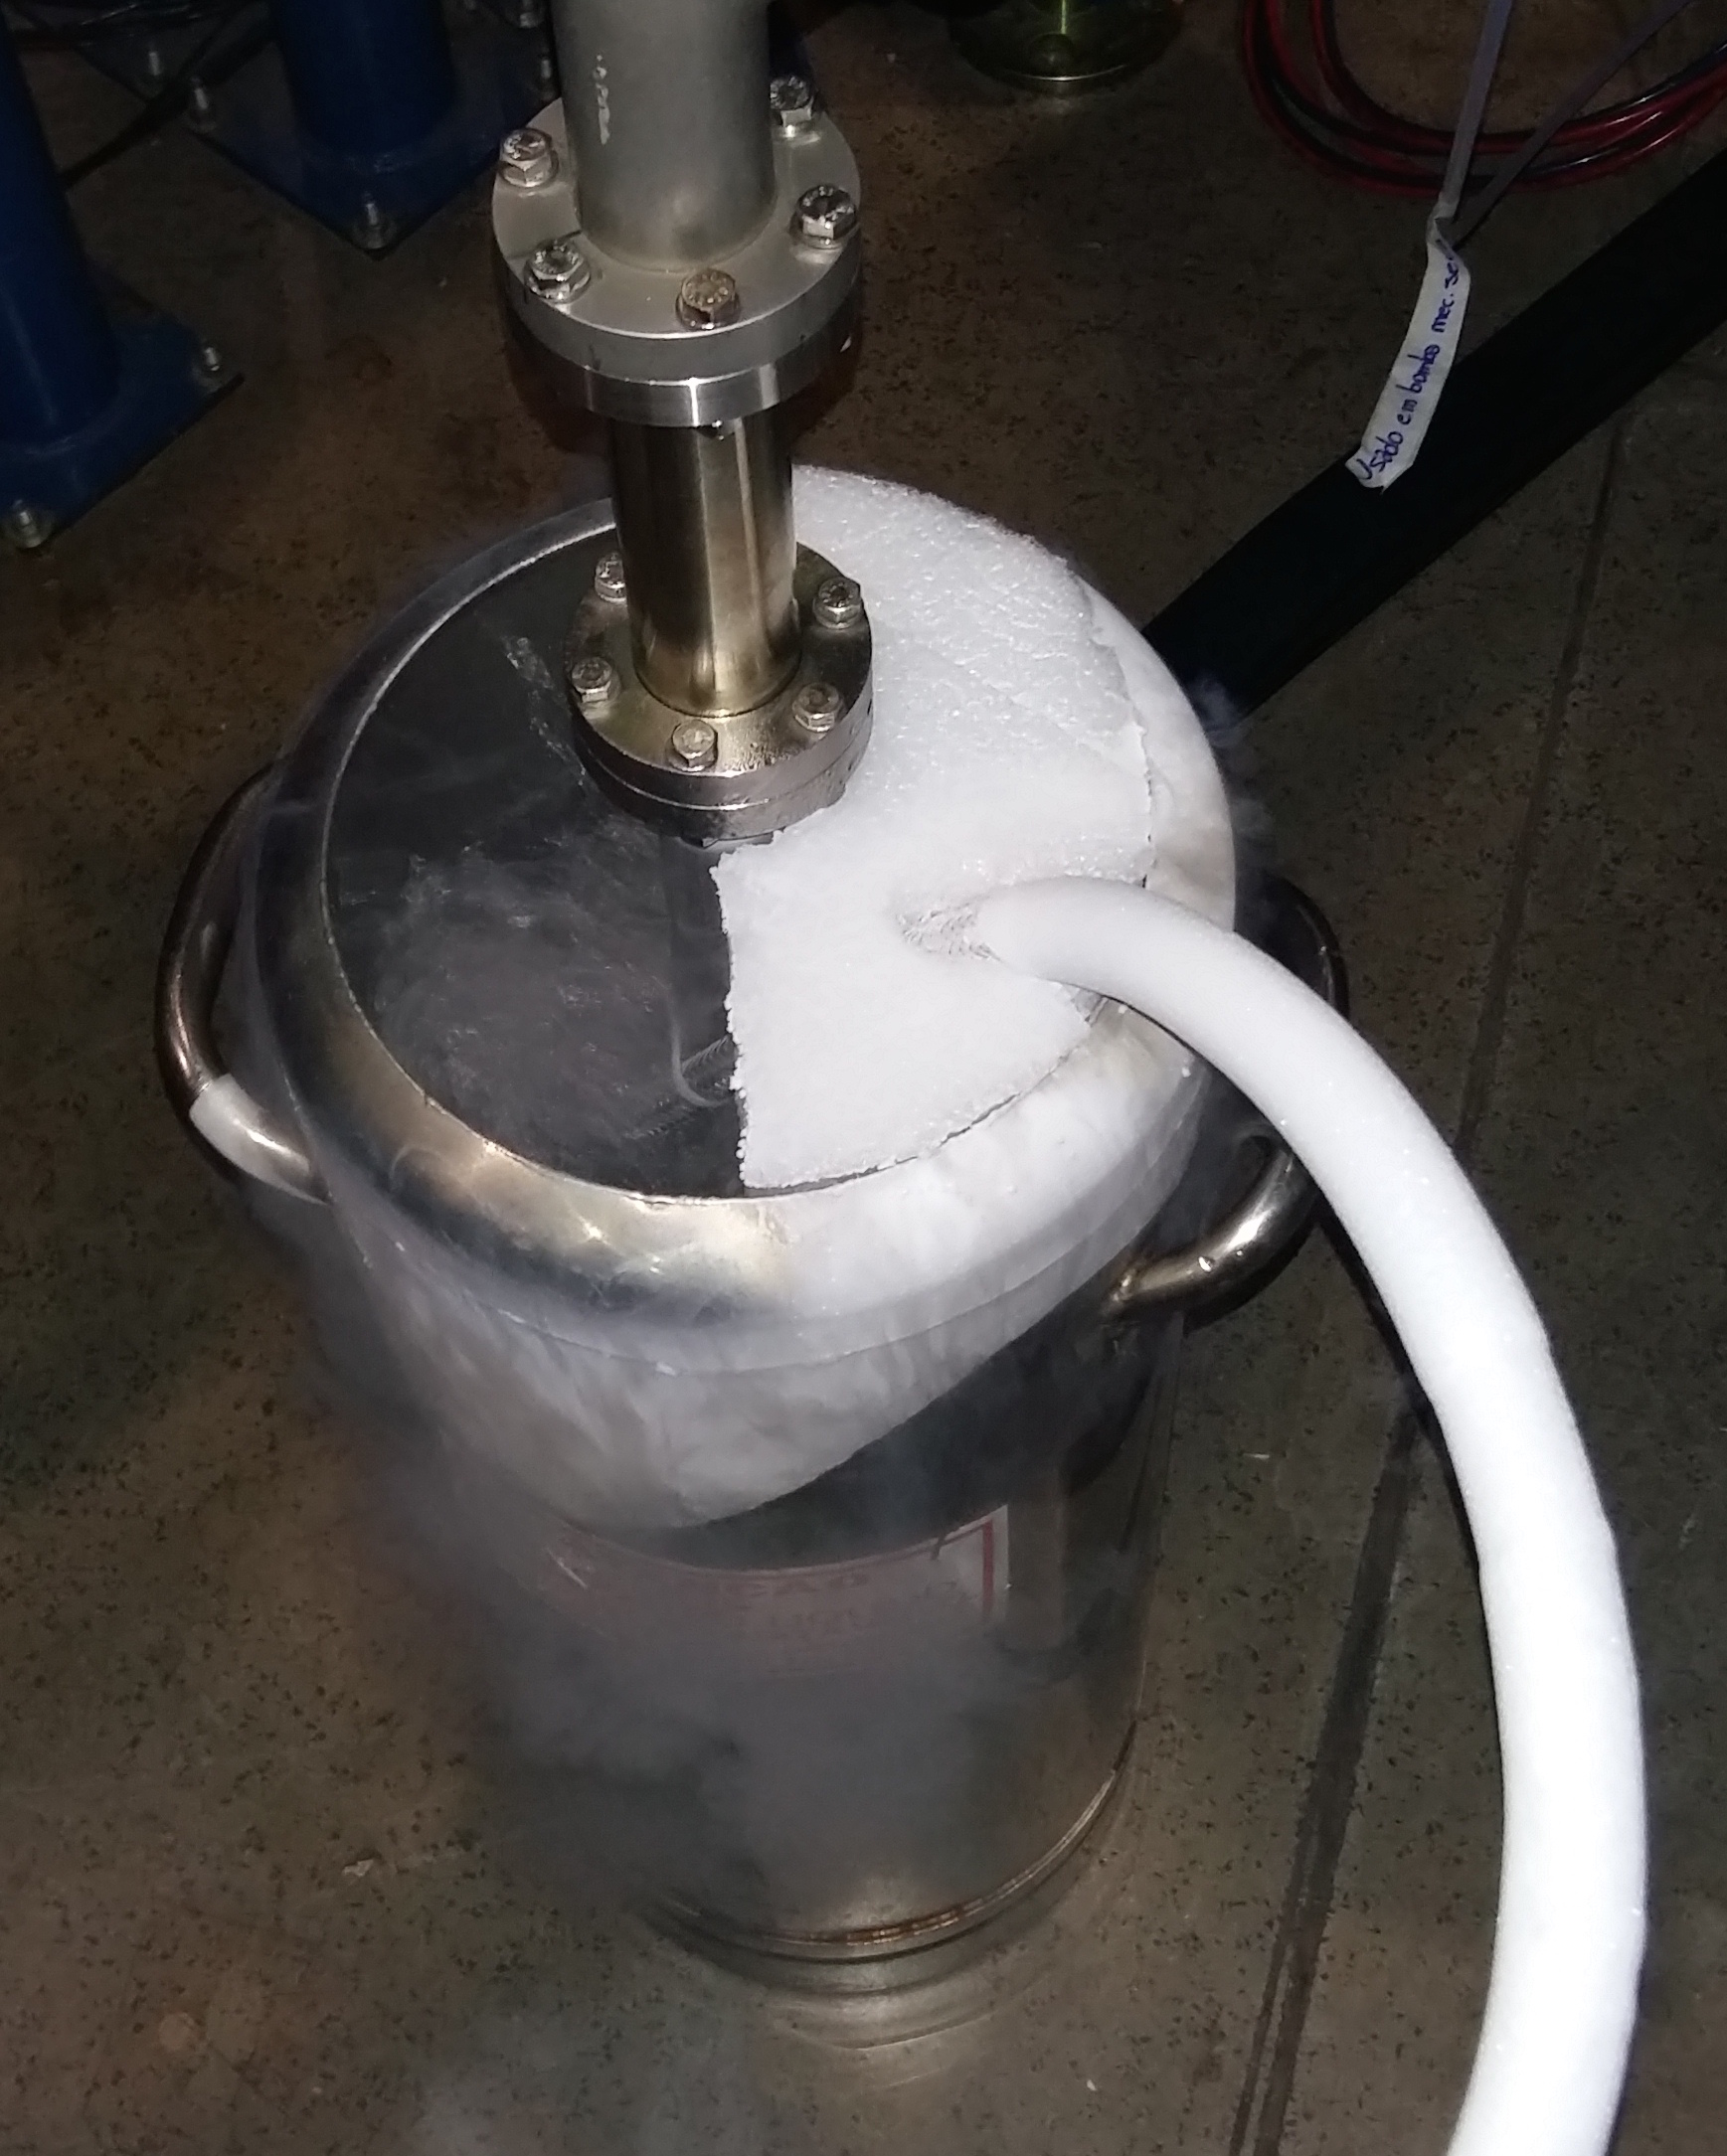
\includegraphics[height=6cm]{pds-tgm_0}
\end{dunefigure}


The detection efficiency of the ARAPUCA was calculated by  determining the number of photoelectrons detected corresponding to the end point of the $\alpha$ spectrum and comparing it with the expected number of photons impinging on the acceptance window for that  particular energy value ($\sim$4.3 MeV).  This depends only on known properties of \lar and on the solid 
angle subtended by the ARAPUCA window. A detection efficiency at the level of 1.8\%  was measured, consistent with \dword{mc} expectations for the this configuration\cite{Marinho:2018doi}.

%\subsubsection{Measurements performed at FERMILAB}
%\label{subsec:test_fnal}

The next several prototypes were tested under cryogenic conditions at Fermilab.  
The first, performed in mid-2016 at the Proton Assembly Building (PAB) at the ScENE cryogenic test facility, had dimensions of  \SI{5.0}{cm}$\times$\SI{5.0}{cm}$\times$\SI{1.0}{cm} with a dichroic window of \SI{5.0}{cm}$\times$\SI{5.0}{cm} with a cut-off of \SI{400}{nm} which was deposited with pTP and \dword{tpb}. However, in this case, two of sensL \dwords{sipm} mod C60035 were installed inside the box.  The ARAPUCA was again deployed inside a vacuum-tight cryostat filled with ultrapure \lar. An $^{241}$Am alpha source was positioned in front of the window of the device \SI{5}{cm} from its center. The efficiency of the ARAPUCA was estimated taking into account that the alpha particles from this source have a  monochromatic energy of about \SI{5.4}{MeV}. 
The estimated efficiency in this case was approximately 1\%, a factor two below the expected value; this is attributed to the sub-optimal quality and uniformity of the pTP and \dword{tpb} films, and to the lack of reflectivity of the inner PTFE surfaces in this early prototype.
%\fixme{was the "sub-optimal quality" based on a visual inspection or other determination?}

The next set of tests was performed at the beginning of 2017 at the PAB, but using the \dword{tallbo} facility, which is large enough to allow testing of several devices at a time. Eight different ARAPUCA cells with filters from different manufacturers, different reflectors, and different dimensions were tested.  Scintillation light was again produced by alpha particles emitted by an $^{241}$Am  source mounted on a holder that could be moved with an external manipulator in order to place it in 
front of each prototype. The detection efficiencies of these ARAPUCAs ranged from 0.4\% to 1.0\%.
%\fixme{Are these the correct values to use?}

The most recent measurements were performed in the \dword{tallbo} facility at the end of 2017 with an array of eight ARAPUCAs together with two reference bars (double-shift light guide design. The data analysis for the ARAPUCA array is currently underway. 
% 4/10/18 rjw \fixme{Any updates that we can include?}

%\end{enumerate}

\subsubsection{ARAPUCA in ProtoDUNE-SP}

Two arrays of ARAPUCA modules will be operated inside \dword{pdsp} to test the devices in a large-scale experimental environment and allow direct comparison of their performance with the light guide designs. 
%The first array has been installed in the \dword{apa} \#3, while the second one will be installed in the \dword{apa} \#6.
 
Each \dword{pdsp} ARAPUCA module array is composed of sixteen cells where each cell is an ARAPUCA box with dimensions of \SI{8}{cm}$\times$\SI{10}{cm}; half of the cells have twelve \dwords{sipm} installed on the bottom side of the cell and  half have six \dwords{sipm}. The \dwords{sipm} have active dimensions \SI{0.6}{cm}$\times$\SI{0.6}{cm} and account for 5.6\% (\num{12} \dwords{sipm}) or \num{2.8}\% (\num{6} \dwords{sipm}) of the area of the window (\SI{7.8}{cm}$\times$\SI{9.8}{cm}).
The \dwords{sipm}  are passively ganged together, so that only one readout channel is needed for each ARAPUCA grouping of \num{12} \dwords{sipm} (the boxes with six \dwords{sipm} are ganged together to form \num{12}-\dword{sipm} units) so a total of \num{12} channels is required per array. Studies are underway to investigate active ganging that would permit combining signals from multiples boxes as required to reduce the number of electronics channels and cables (currently in the \dword{spmod} \SI{10}{kt}, we anticipate being restricted to four readout channels per \dword{pd} module). 
The total width of a module is \SI{9.6}{cm}, while the active width of an ARAPUCA is \SI{7.8}{cm}, the length is the same as the light guide modules ($\sim$\SI{210}{cm}). 
The first ARAPUCA array installed in \dword{pdsp} is shown in Figure~\ref{fig:arapuca_array}. If the ARAPUCA cells achieved the same detection efficiency as earlier prototypes (1.8\%), the effective area of an ARAPUCA module will be approximately \SI{23}{cm$^2$}.

%\begin{dunefigure}[Drawing of two ARAPUCAs of the design used for \dword{pdsp}.]{fig:arpk}
%{Drawing of two ARAPUCAs in one modular unit, each one read-out by 12 \dwords{sipm}; this design was used for \dword{pdsp}.} 
%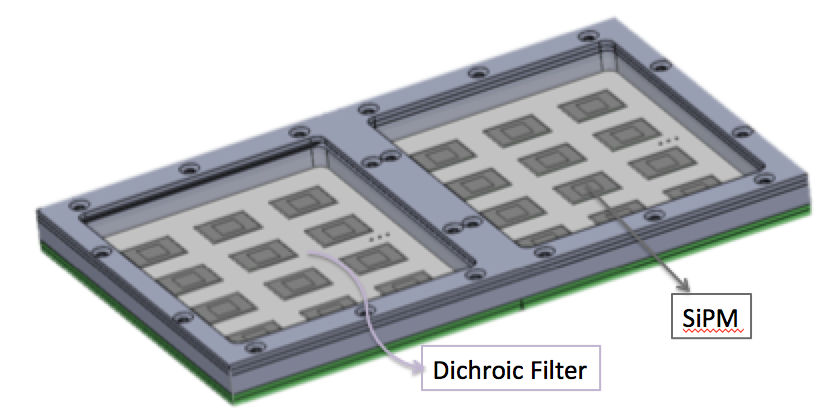
\includegraphics[height=4cm]{pds-arapuca}
%\end{dunefigure}

\begin{dunefigure}[Full-scale ARAPUCA for \dword{pdsp} during assembly.]{fig:arpk}
{Full-scale ARAPUCA for \dword{pdsp} during assembly. \dwords{sipm} are visible in the sixteen cells before the installation of reflecting foils, coated filter windows, and readout cabling. } 
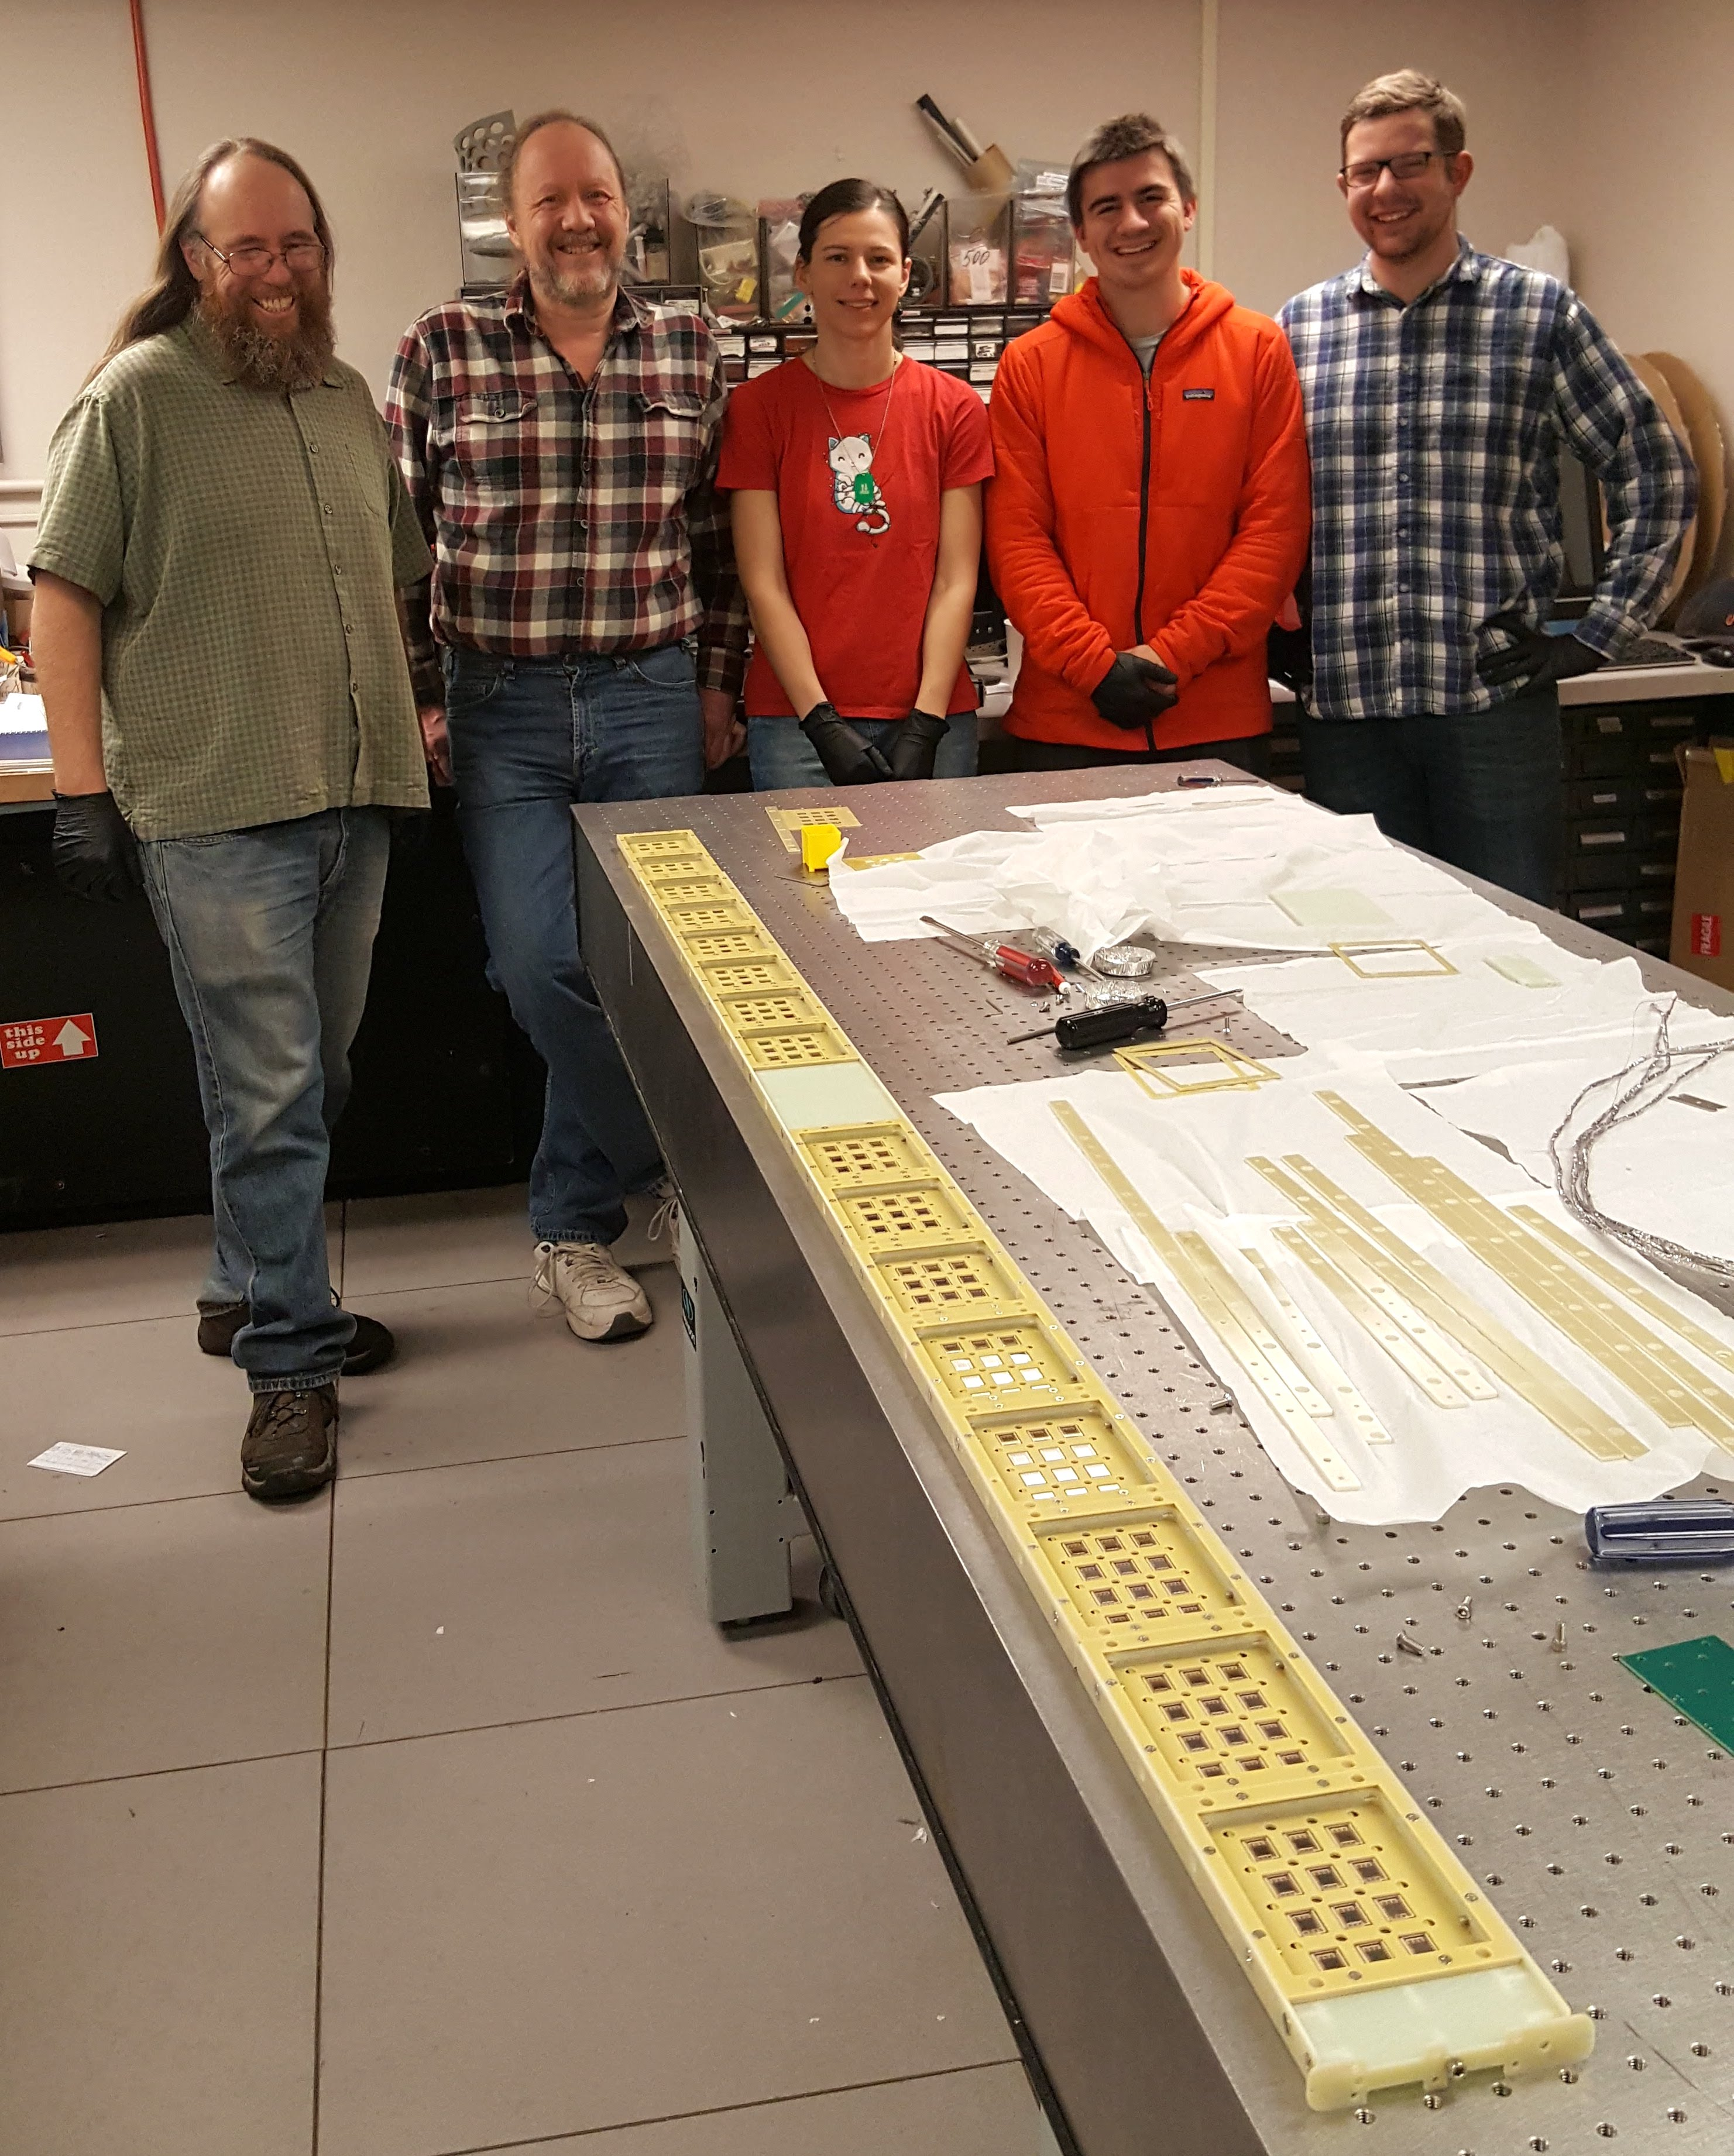
\includegraphics[height=9cm]{pds-arapuca-assembly.jpg}
\end{dunefigure}

\begin{dunefigure}[ARAPUCA array in \dword{pdsp}.]{fig:arapuca_array}
{ARAPUCA array in \dword{pdsp}.} 	
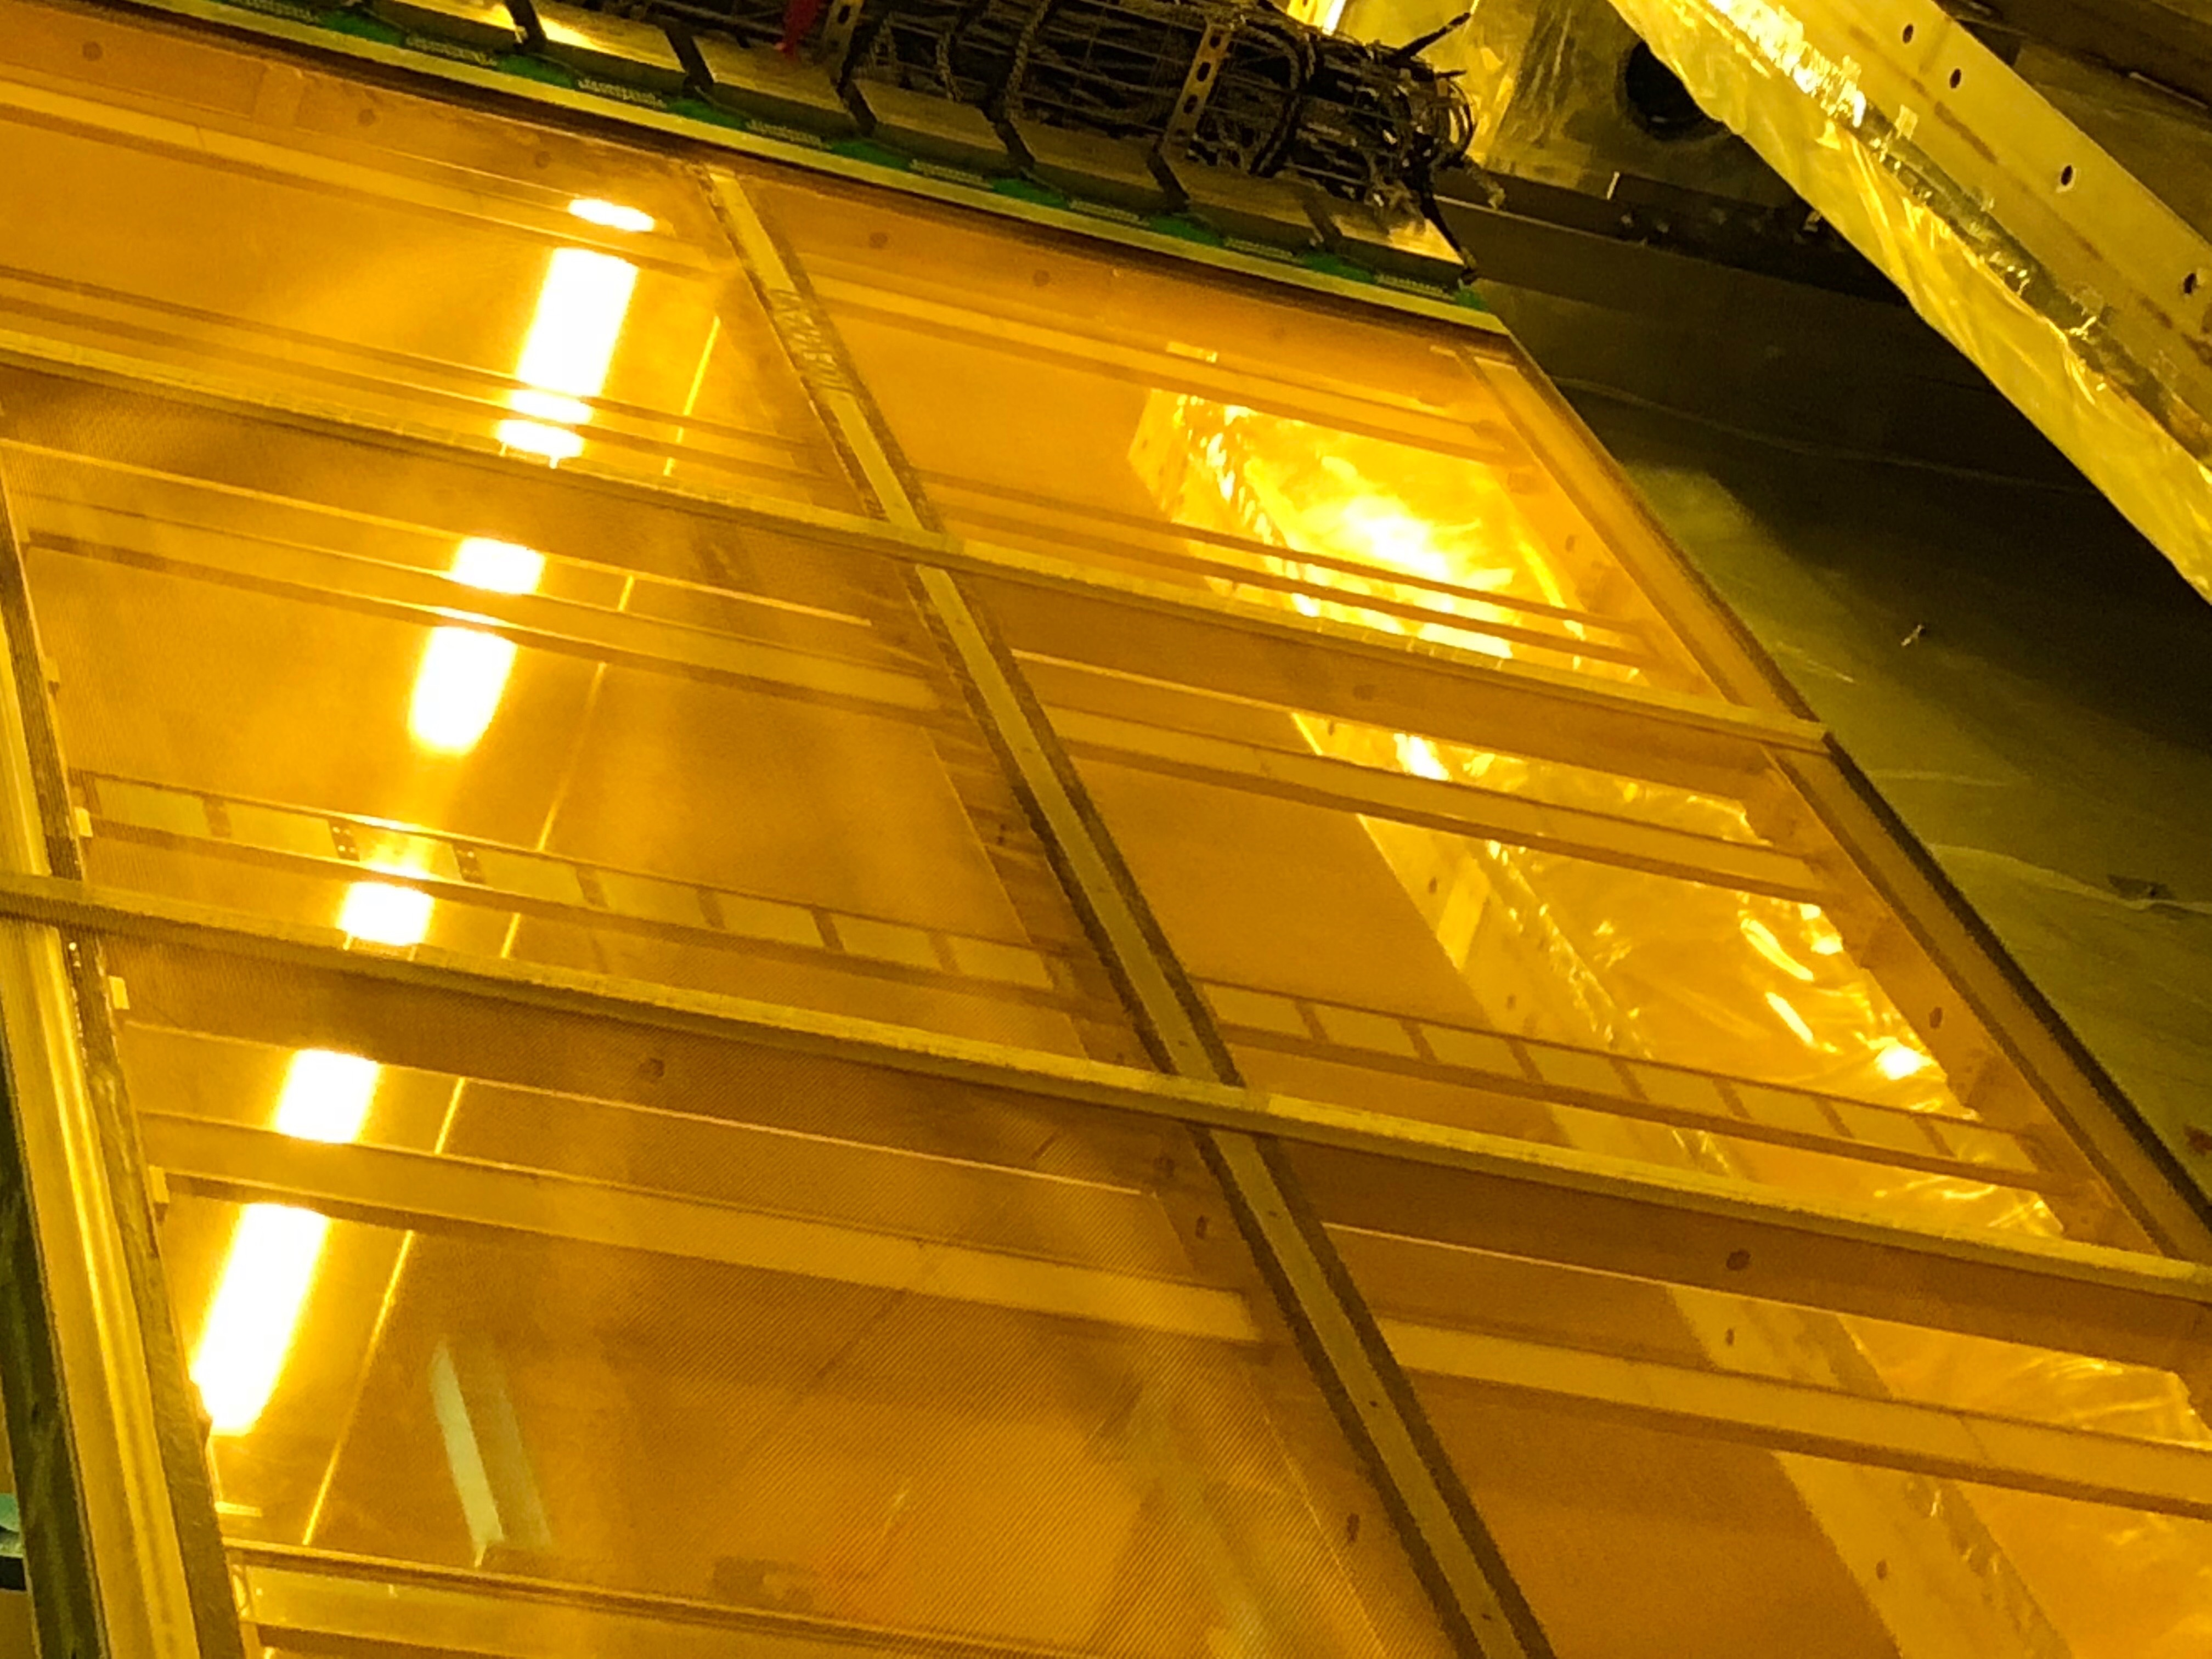
\includegraphics[height=8cm]{pds-arpk-apa3_pd.jpg} 
\end{dunefigure}
%***********************************************************************%

%The ARAPUCA device is undergoing an intense R\&D program that aims to establish its 
%viability as the photon detection system for the single phase DUNE far detector, both 
%in terms of demonstrating an absolute detection efficiency of several percent and with respect to long term reliability.

\subsubsection{X-ARAPUCA} 
\label{sssec:x-arapuca}
X-ARAPUCA represents  an alternative line of development with the aim of further improving the collection efficiency, while retaining the same working principle, mechanical form factor and active  photo-sensitive coverage. X-ARAPUCA is effectively a hybrid solution between the ARAPUCA and the wavelength-shifting light guide concepts, where photons trapped in the ARAPUCA box are shifted and transported to the readout via total internal reflection in a short light guide placed inside the box.
This solution minimizes the number of reflections on the internal surfaces of the box and thus the probability of photon loss. Simulations suggest that this modification will lead to a rather significant increase of the collection efficiency, to around 60\%, so the photon detection efficiency including the \dword{sipm} response could approach 20\%. 

 \begin{dunefigure}[X-ARAPUCA design: assembled cell (left),  exploded view (right).]{fig:pds-x-arapuca-cell}
{X-ARAPUCA design: assembled cell (left),  exploded view (right). The size and aspect ratio of the cells can be adjusted to match the spatial granularity required for a \dword{pd} module.}
 % \vspace{-2.5cm}
 %two-sided x-arapuca 4/14/18
  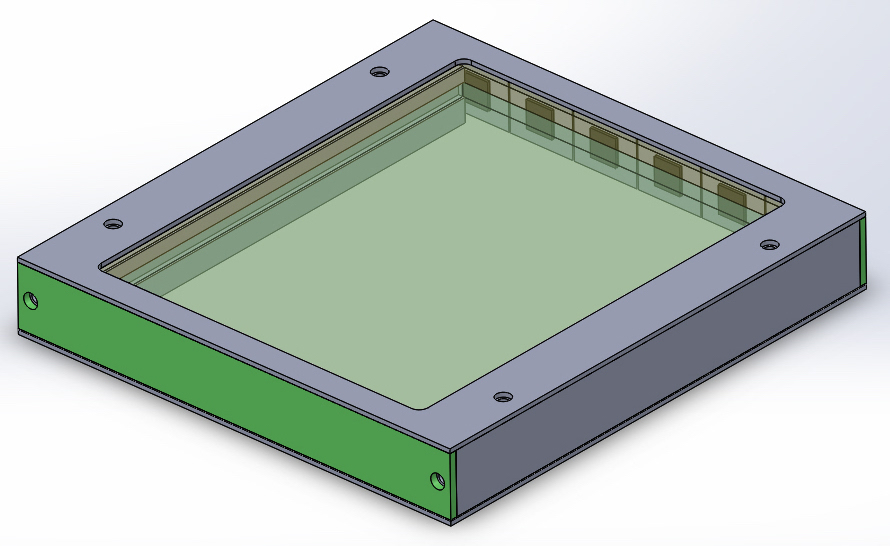
\includegraphics[height=.25\textheight]{pds-x-arapuca-cell}
  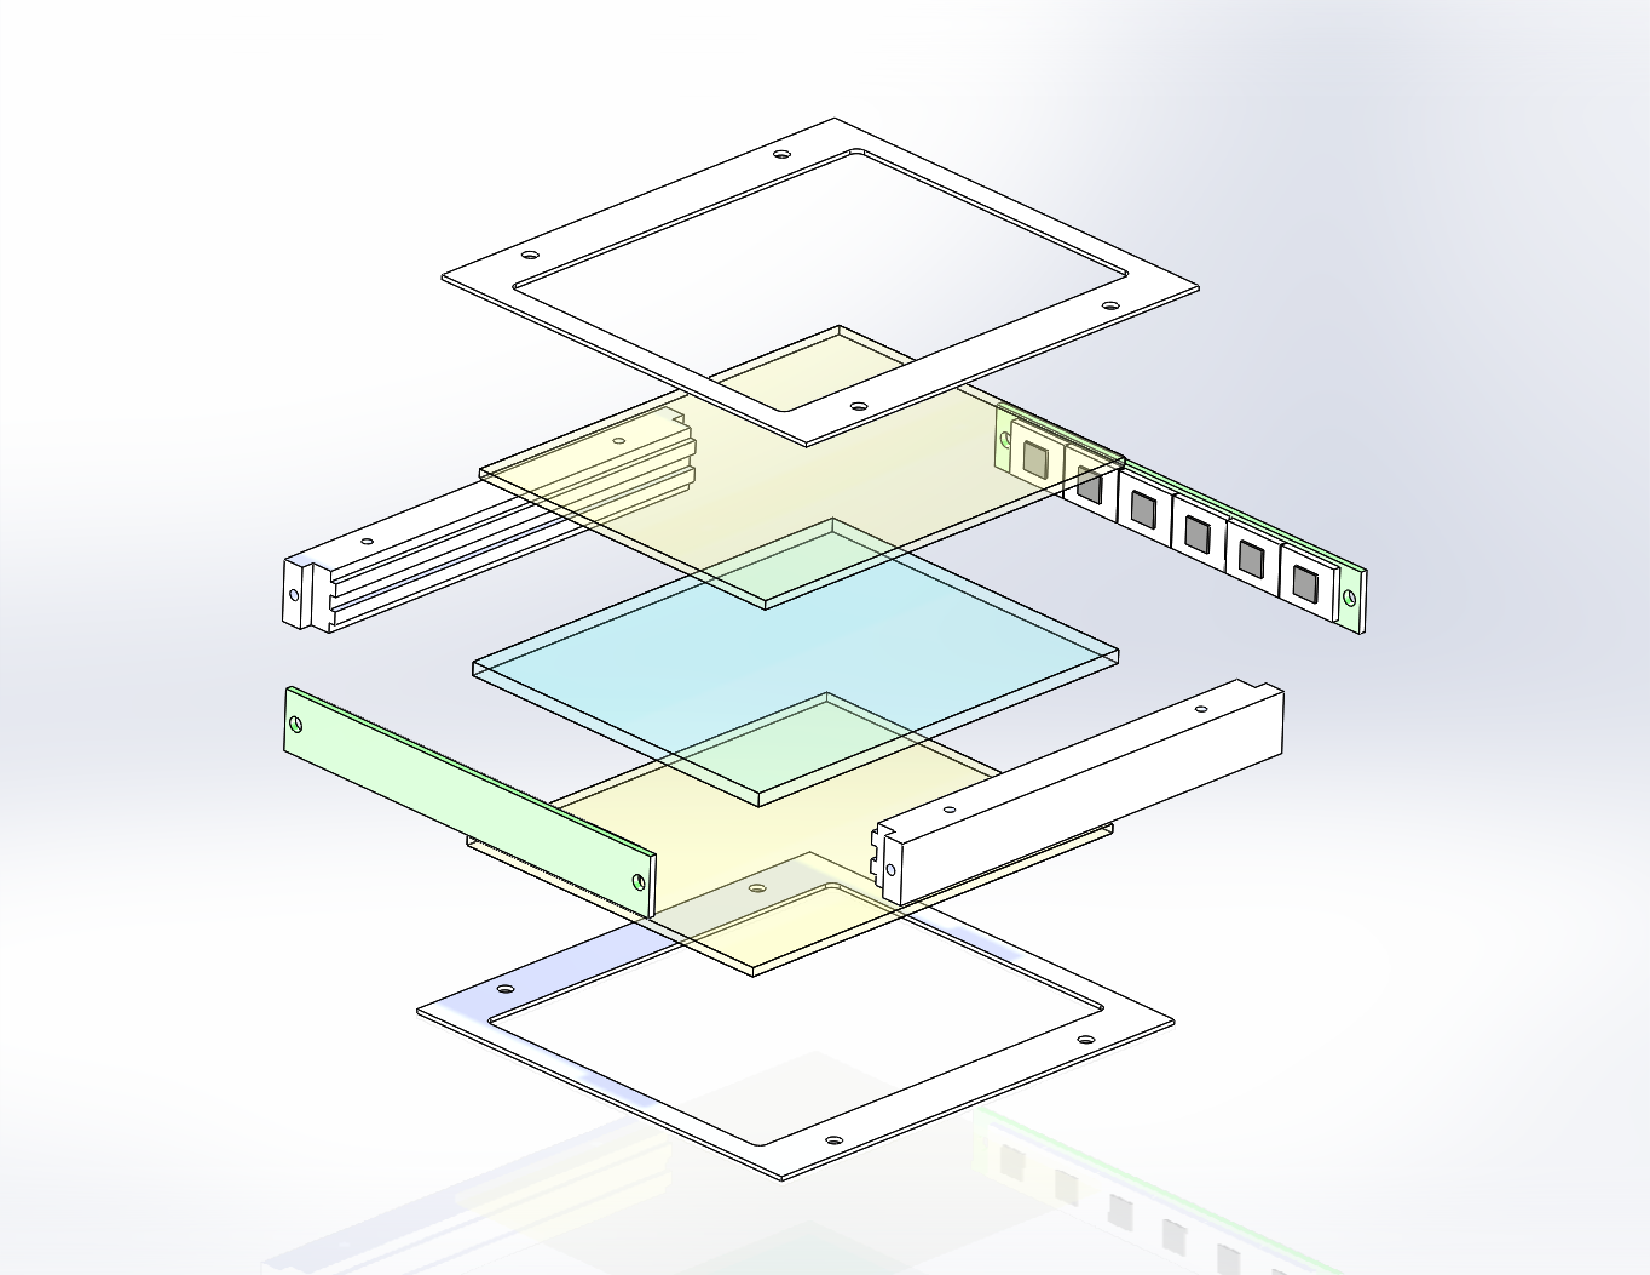
\includegraphics[height=.25\textheight]{pds-x-arapuca-exploded-view}
\end{dunefigure}

% In a standard ARAPUCA the photon trapping effect is obtained by means of a dichroic filter and a two-steps wavelength shifting process, %the first from \dword{vuv} to UV outside the acceptance window of the box and the second inside from UV to blue, across the filter cutoff. Double %shifted photons are eventually collected by an array of photosensors (\dword{sipm}) distributed on the backplane of the box, opposite to the the %acceptance window. 

In the X-ARAPUCA design, Figure \ref{fig:pds-x-arapuca-cell}, the inner shifter coating/lining over the reflective walls of the box is replaced by a thin wavelength-shifting light guide slab inside the box, of the same dimensions of the acceptance filter window and parallel to it. The \dword{sipm} arrays are installed vertically on the sides of the box, parallel to the light guide thin ends. 
 In this way a fraction of the photons will be converted inside the slab and guided to the readout, other photons,  e.g,. those at small angle of incidence below the critical angle of the light guide slab, after conversion at the slab surface will remain trapped in the box and eventually collected as for the standard ARAPUCA.
 
 A full-sized X-ARAPUCA prototype is under development. The light guide is a \SI{3}{mm} thick \dword{tpb}-doped acrylic plate. Two readout boards, each with several passively ganged \dwords{sipm} in a strip configuration, are mounted along the thin edges of the box and their ganged signals are combined into a single channel readout. 
 The aspect ratio of the cells can be adjusted to match the required spatial granularity for the \dword{pd} module.
 
 %  V2 - text below aded to v1 - FC 22feb18 %%%%%%%%%%%%%%%%%%%%%%%%%%%%%%%%%%%
 %% Drop this until is it further developed rjw 16mar18
 %
% A variant of the approach to the dipped-bar \dword{pd} option described in the preceding section, 
% that might also have application in the X-ARAPUCA \dword{pd} configuration,
% would be to use the now conventional extruded-scintillator process.  Standard extruded scintillator bar (like that
%used in MINOS) has a core of polystyrene and a cladding of acrylic.  The core is doped with
%a primary dopant (often p-terphenyl) and a wavelength shifter (WLS).  The cladding, in the case of
%MINOS, was doped with a reflector, TiO$_2$.  For the DUNE \dword{pds}, the primary dopant would
%be moved to the cladding and over-doped (3-5\% by wt.) and no reflector would be used.  The cladding polymer would be a
%high-grade acrylic.  The polystyrene core would be doped with the desired WLS.   The very-high
%doping level in the cladding would mean that p-terphenyl molecules would be separated by only 
%$\simeq 1~\mathrm{\AA}$, so the p-terphenyl in the acrylic can effectively absorb the UV
%photons.  A reflector layer could be added to the three faces not facing the \lar. 
%The potential advantages of this variant are expected to be in a 
%better uniformity, stability, well established and low-risk process, and cost.
%
%%%%%%%%%%%%%%%%%%%%%%%%%%%%%%%%%%%%%%%%%%%%%%%%%%
 
\subsubsection{ARAPUCA Configuration in DUNE \SI{10}{kt} }
\label{sssec:arapuca-dune}

The modular arrangement of the \dword{spmod} TPC calls for a configuration across the width of the cryostat starting with an \dword{apa} plane against one cryostat wall, and following with \dwords{apa} and \dwords{cpa} arranges as follows:  APA-CPA-APA-CPA-APA. This means that the central \dword{apa} will collect charge and see scintillation light from \lar volumes on both sides, whereas those by the wall collect from only one side.  
While the ARAPUCA modules deployed in \dword{pdsp} collect light from only one direction, several ARAPUCA configurations under development are capable of collecting light from both sides (including the X-ARAPUCA concept).
The optimal configuration of ARAPUCA modules has not yet been determined, but the basic design allows for both single-sided and double-sided cells with no impact on the \dword{apa} design.


%==========================================================================================

\subsection{Photon Collector: Dip-Coated Light Guides}
\label{ssec:fdsp-pd-pc-bar1}
%\metainfo{\color{red} \bf Content needed: (4 pages) Toups}

%\subsubsection{Description}

The \textit{dip-coated} light guide design is mechanically the simplest of the three options. Figure~\ref{fig:pds-dippedbarpic} illustrates the process by which \lar scintillation photons are converted and detected in this approach.  \dword{vuv} scintillation photons incident on the bar are absorbed and wavelength-shifted to blue ($\sim$\SI{430}{nm}) by the \dword{tpb}-based coating on the surface of the bar.  A portion of this light is captured in the bar and guided to one end through total internal reflection where it is detected by an array of \dwords{sipm}, whose PDE is well-matched to the blue light.  Dimensions of the bars in \dword{pdsp} are: \SI{209.3}{cm}$\times$\SI{8.47}{cm}$\times$\SI{0.60}{cm}.
Since the bar is coated on all sides, in the \dword{spmod} it can be employed both in the wall \dwords{apa} as well as in the center \dword{apa} array where scintillation light approaches from two drift volumes.

\begin{dunefigure}[Schematic of scintillation light detection with dip-coated light guide bars.]{fig:pds-dippedbarpic}
{Schematic of scintillation light detection with dip-coated light guide bars.}
  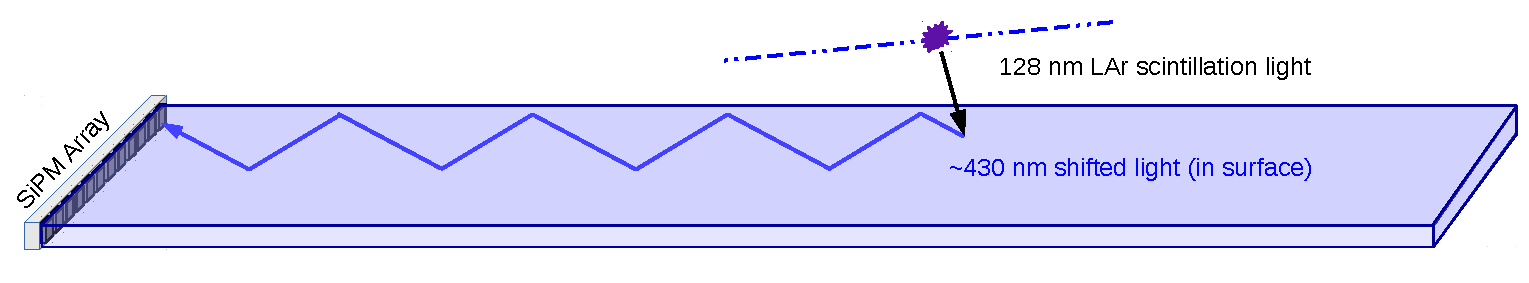
\includegraphics[width=0.8\columnwidth]{pds-dipcoatlg-cartoon}
\end{dunefigure}

%\subsubsection{Testing and Performance}

The dipping process and coating formula have undergone a series of development iterations~\cite{Moss:2014ota},
%\cite{Z. Moss et al 2015 JINST 10 P08017, Z. Moss et al 2016, arXiv:1604.03103v1}, 
with the bars undergoing extensive testing at both room and cryogenic temperatures.
As a part of the production process, the attenuation of each dip-coated light guide bar is measured at room temperature in a dark box with a UV LED; 80\% of the bars measured have an attenuation length in air of \SI{6}{m} or greater.   
Attenuation measurements on full-length bars have not yet been performed in \lar, but a model presented in ~\cite{Moss:2014ota} predicts effective attenuation lengths greater than \SI{2}{m}~\cite{Moss:2016yhb}.  The general features of this model were validated by measurements using $^{210}$Po alpha sources in the \dword{tallbo} cryogenic test stand at \dword{fnal}.
%\cite{ Z. Moss et al 2016 atXiv 1604.03103}.  
%These tests also validated a model for predicting dip-coated light guide bar attenuation lengths in \lar based on measurements of attenuation lengths at room temperature, which are much easier to perform.  

A further validation of the bar performance came from a set of measurements taken in the \dword{tallbo} cryostat containing the four initial candidate photon collector technologies using alpha sources and tracked cosmic ray muons, allowing side-by-side comparisons~\cite{Whittington:2015rkr}.  As a result, the two approaches that showed the highest promise, dip-coated and double-shift light guides (described in the next section), were continued for further development since these had similar photon detection efficiency, $\sim$0.1\%, that was significantly higher than the other two. 
%It is hoped to repeat these tests in the near future to extract the overall efficiency by comparing the number of photoelectrons detected at the end of the bar to the number of photons from the alpha source incident on the surface of the bar.

%\subsubsection{Performance}

%Tests of the dip-coated light guide bars in the \dword{tallbo} cryostat with alpha sources indicate that the attenuation length of the bars in \lar %is $>2$ m.  Data using tracked cosmic muons in \dword{tallbo} indicated that the dip-coated bars have comparable or better performance than the %other candidate photon detection technologies prototypes~\cite{whittington-2016}.
%Tests of the dip-coated light guide bars in the \dword{tallbo} cryostat with alpha sources and tracked cosmic muons
%indicate that the attenuation length of the bars in \lar is $>2$ m~\cite{whittington-2016}.
%% illegal syntax: \cite{D. Whittington 2016 JINST 11 C05019}.


%\subsubsection{Potential Improvements for the DUNE Far Detector}

%There are two areas of potential improvements to the dip-coated light guide bars: improving the coating performance and enhancing the readout of the light guide bars.  Test bars have been produced with a higher \dword{tpb}-to-acrylic ratio, which may have a higher conversion efficiency without sacrificing a reduction in attenuation length.  A straightforward improvement under consideration is to read out both ends of the  bar rather than a single end as is the case for bars deployed in \dword{pdsp}.  This improvement could increase the photon detection efficiency of the dip-coated light guide bars by up to a factor of two.

 A simple improvement to the bar performance is to read out both ends of the bar rather than a single end as is the case for bars deployed in \dword{pdsp}.  
In addition, test bars have been produced with a higher \dword{tpb}-to-acrylic ratio, which may have a higher conversion efficiency without introducing a reduction in attenuation length. These improvements could increase the photon detection efficiency of the dip-coated light guide by more than a factor of two.

%==========================================================================================
\subsection{Photon Collector: Double-Shift Light Guides}
\label{ssec:fdsp-pd-pc-bar2}
%\todo{\color{blue} Content: Whittington}
%Update DW 2/23/18

In the early implementations of the dip-coated light guide development there was a strong dependence of the light yield along the length of the bar, presumed to be due to the impact of the coating on the total internal reflection efficiency.  In an effort to mitigate this effect, the \textit{double-shift} light guide design decouples the process of converting \dword{vuv} photons to optical
wavelengths from the transportation of photons along the bars. This is achieved by positioning an array of acrylic plates coated with \dword{tpb} in front of a high-quality commercial polystyrene light guide doped with a second wavelength-shifting compound.

%\subsubsection{Description}

Figure~\ref{fig:pds-doubleshiftlg-cartoon} illustrates the double-shift light guide concept. \dword{vuv} scintillation photons incident on the acrylic plates are converted to blue wavelengths ($\sim$\SI{430}{nm}) and a fraction of these blue photons penetrate the light guide and are converted to green ($\sim$\SI{490}{nm}). The re-emission of these green photons, taken to be a Lambertian distribution (isotropic luminance), leads to some becoming trapped by total internal reflection within the light guide and  transported to the end of the light guide where they are detected by an array of \dwords{sipm}.

\begin{dunefigure}[Schematic of the principle of a double-shift light guide.]{fig:pds-doubleshiftlg-cartoon}
{Schematic of the principle of a double-shift light guide.}
  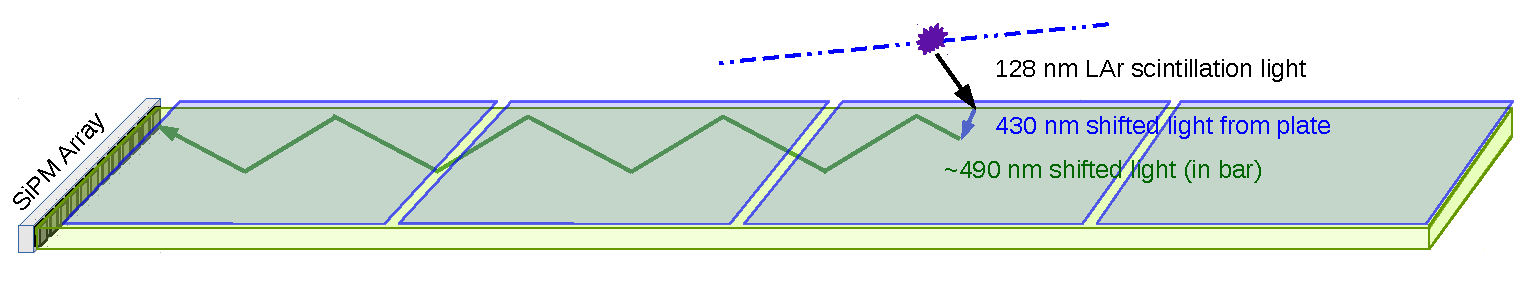
\includegraphics[width=0.8\columnwidth]{pds-doubleshiftlg-cartoon.pdf}
\end{dunefigure}


%\begin{itemize}
%\item Wavelength-Shifting Plates: Acrylic spray-coated with \dword{tpb}. \fixme{\dword{tpb} absorption and emission properties.}
%\item Wavelength-Shifting Light Guide: EJ-280 light guides manufactured by Eljen Technologies\footnote{http://%www.eljentechnology.com}. \fixme{EJ-280 absorption and emission properties. PDE of \dwords{sipm}.}
%
%\end{itemize}

%\subsubsection{Wavelength-Shifting Plates}

%The wavelength shifting compound tetraphenyl-butadiene\footnote{1,1,4,4-tetraphenyl-1,3-butadiene} (\dword{tpb}) is commonly used to convert %scintillation light from liquid noble elements to visible wavelengths. \dword{tpb} emits visible photons typically between 420~nm and 450~nm. 
The radiator plates are formed by spray-coating \dword{tpb} on the outer surface of acrylic plates, as described in Section~\ref{ssec:fdsp-pd-pc-prod-bar2}.
A full-scale double-shift light collector module consists of six radiator plates mounted on each face of the wavelength-shifting light guide (12 plates total). The \SI{210}{cm}$\times$\SI{8.6}{cm} light guide is fabricated by Eljen Technologies\footnote{http://www.eljentechnology.com} and consists of a polystyrene bar doped with the EJ-280 wavelength shifter. 
EJ--280 features an absorption spectrum that is well matched to the \dword{tpb} emission spectrum so wavelength-shifted photons emitted from the plates are absorbed with good efficiency. 
% and the re-emitted green light (480-510~nm), are transported down the light guide by total internal reflection. 
%\subsubsection{Wavelength-Shifting Light Guide}
%A portion of the photons emitted by the \dword{tpb} radiator plates impinge on an EJ-280 light guide manufactured by Eljen Technologies\footnote{http://www.eljentechnology.com}. 
%This is a commercially-fabricated polystyrene light guide doped with a second wavelength shifter. The EJ-280 wavelength shifter features an absorption spectrum that is well matched to the \dword{tpb} emission spectrum. Absorbed photons are then re-emitted with typical green wavelengths in the range 480~nm to 510~nm.
%\subsubsection{Photodetectors}
%At the end of the bar, the green light is detected by an array of \dwords{sipm}; 

For most of the testing and the \dword{pdsp} modules,  the \dword{sipm} array used \SI{0.6}{cm}$\times$\SI{0.6}{cm} sensL C-series MicroFC-60035-SMT \dwords{sipm}. These were originally selected since they were a good match for the \dword{tpb} emission spectrum on the dip-coated bars. However, they have a photon detection efficiency between 20\%--35\% across the emission spectrum of the EJ-280 wavelength shifter, compared to up to 40\% at the peak, so selecting a different device with a better-matched photon detection efficiency would improve the  performance of the double-shift design.

%\subsubsection{Testing and Performance}

The double-shift light guide design has undergone a series of development iterations to improve its performance, carried out at Indiana University (IU) and at Fermilab's cryogenic and vacuum test facility in the PAB. Comparative testing of light guide designs at PAB in mid-2015 demonstrated the viability of the double-shift light guide concept~\cite{bib:JINST-11-C05019}. 
An improved design similar to that deployed at \dword{pdsp} was studied at the Blanche test stand at Fermilab in September of 2016 with a complementary component-wise analysis program at IU afterward, as detailed in \cite{bib:DoubleShiftLG-NIM-171113}. The attenuation characteristics of this light guide were measured at IU, while the  detection efficiency for incident \lar scintillation photons was measured with a vacuum-ultraviolet (\dword{vuv}) monochromator at IU and using scintillation light from cosmic rays at the Blanche test stand.

%\subsubsection{Performance}

Analysis of the double-shift light guide's attenuation properties determined an attenuation profile in \lar characterized by a double-exponential function of the form $f(z) = A \exp(-z/\lambda_{A}) + B \exp(-z/\lambda_B)$ with $z$ the distance from the instrumented end and parameters $A = $0.29, $\lambda_A = $4.3~cm, $B = $0.71, and $\lambda_B = $225~cm~\cite{bib:DoubleShiftLG-NIM-171113}. The effective attenuation length of $\sim$\SI{2}{m} is comparable to the width of an \dword{apa} when the double-shift light guide is deployed in \lar.

%\fixme{what is the measured central value and spread if known on more than one bar?}

Using both direct measurement with the monochromator and scintillation light, the photon detection efficiency of this detector was determined to be 0.48\% at the end close to the \dword{sipm} readout. The total effective area for detecting \dword{vuv} scintillation photons in this module can be determined by integrating the product of this efficiency and the attenuation function over the area of the detector:
\begin{equation*}
  A_{eff} = (0.0048) (8.5\text{cm}) \int_{0\text{cm}}^{210\text{cm}} \hspace{-2em}dz \left( 0.29 \exp(-z/4.3\text{cm}) + 0.71 \exp(-z/225\text{cm}) \right)
\end{equation*}
This corresponds to an effective area for detecting \dword{vuv} scintillation photons of 4.1 cm$^{2}$ per module per drift volume, which corresponds to overall 0.23\% photon detection efficiency for events occurring on one side of the \dword{apa}.
Since the radiator plates are deployed on both faces of the light guide, modules in the center \dword{apa} array are sensitive to scintillation light from the two drift volumes on either side. 
% and modules in the outer arrays are able to detect scintillation light originating outside of the TPC volume, if this is desirable (they can be masked, if not).

%DWW 16mar18 start %%%%%%

%Moved from above dww

%\subsubsection{Potential Improvements for final design}

There are several ways that the current design could be improved. The double-shift light guide deployed in the \dword{pdsp} \dwords{apa} is constrained to read out at a single end. Proposed changes to the \dword{apa} size and cabling routing scheme for the \dword{spmod} would allow for a second array of \dwords{sipm} at the opposite end of the light guide, which would almost double the performance of the photon detection system.
A \dword{sipm} with a wavelength-dependent PDE that is better matched to the EJ-280 emission spectrum would also improve the efficiency. Simulations of the transport of light within the light guide suggest that applying a highly reflective coating to the long, narrow inactive sides of the light guide would improve the attenuation function and increase the effective area of the light guide module. These effects combined lead to a potential increase of the effective area up to four times the current prototypes, approaching 1\% detection efficiency.
%to 16 cm$^{2}$ per module per drift volume.

%As is illustrated in Figure~\ref{fig:pds-sn-eff-simulation}, the simulated supernova neutrino detection capability of a photon detection system based on this %module depends strongly on small changes in the estimated efficiency. These potential improvements raise the physics performance in this channel into a %regime where small fluctuations in the module efficiency have a smaller impact on the efficiency to tag these supernova neutrino interactions. These %improvements are an important component to risk mitigation in the photon detection system performance.

%DWW 15mar18 end %%%%%%


%==========================================================================================

\subsection{Additional Techniques to Enhance Light Yield}
\label{sec:fdsp-pd-enh}
%\metainfo{\color{blue} Content: Cavanna/Whittington/Machado}

%>> Start: Andrzej Szelc 14/02/2018 >>>>>>>>>>>>> 
%\subsubsection{\dword{tpb}-Coated Reflector Foils}.   
%%>>rjw Remove as a subsection heading and add a few words of preamble and comment on the concentrator .
% Not a publication, but a proceedings:  To cite this article: Diego Garcia-Gamez and SBND Collaboration 2017 J. Phys.: Conf. Ser. 888 012094

Though we anticipate that the designs described in the previous sections will meet the \dword{pd} performance requirements we do not yet have final designs and so we have also considered options for enhancing the light yield if that becomes necessary. Some of the initial ideas, such as deploying a large array of Winston-cone style reflectors focusing light onto \dwords{sipm} throughout the entire area enclosed by the \dword{apa} frame, would require a significant change in the \dword{apa} production and assembly planning and so will become increasing untenable.  However, one option being investigated in parallel with the photon collector modules design is to convert the scintillation light falling on the cathode plane into the visible wavelengths, which in turn illuminates  photon detectors embedded in the \dword{apa}, as is currently envisioned.

A motivation for this approach is that, due to geometric effects, the baseline PDS design will result in some non-uniformity of light collection along the drift direction. Light emitted from interactions close to the \dwords{apa} has an order of magnitude larger chance of being detected compared to interactions close to the \dword{cpa}. This effect can be mitigated by installing wavelength-shifter (\dword{tpb}) coated dielectric reflector foils on the cathode planes.
Light impinging on these foils is wavelength-shifted into visible wavelengths and reflected from the underlying foils. This light can subsequently be detected by photon detectors placed in the \dwords{apa} provided they are sensitive to visible light (which is not the case for the current photon collector modules). Fig. \ref{fig:ly_with_foils}, shows that if the \dword{apa} photon collectors are capable of recording both direct scintillation light and the visible light from the \dword{cpa}, there is an enhancement of the total light collection close to the cathode (black points), which will increase the detection efficiency in that region. 
Another benefit is the increase in uniformity - this can enable calorimetric reconstruction with scintillation light, which would enhance the charge-based energy reconstruction as well as increase the efficiency of triggering on low energy signals. Introducing the foils on the cathode may also enable drift position resolution  using only scintillation light. This requires the photon detectors to be able to differentiate direct \dword{vuv} light from re-emitted visible light (e.g. two different \dword{pd} detector types) and good enough timing of arrival of first light.

Coated reflector foils are manufactured through low-temperature evaporation of \dword{tpb} on dielectric reflectors e.g. 3M DM2000 or Vikuiti\texttrademark\  ESR. Foils prepared in this manner have been successfully used in dark matter detectors such as WArP\cite{Acciarri:2008kv}. Recently they have been shown to work in LArTPCs at neutrino energies, namely  in the LArIAT test-beam detector \cite{Garcia-Gamez:2017cmu}. In LArIAT they have been installed on the field-cage walls and, during the last run, on the cathode.  

The necessity to record both \dword{vuv} and visible photons in the Photon Collectors would require a change in the current design but is conceptually possible. For example, if the cathode plane were coated with tTP,  some of the ARAPUCA modules could be constructed without the pTP coating on the outer surface of the filter and benefit from the same photon trapping effect but these cells would no longer be sensitive to direct scintillator light.   
Understanding the impact of these competing effects on the physics is under study by the simulation group and the feasibility of coating the cathode with a dielectric medium is being investigated with the DUNE HV consortium.

%This experience has led to the decision to install such foils on the CPA of the SBND detector (a part of the Fermilab  Short-Baseline Neutrino program). 
%In DUNE, the foils would ideally be laminated on the CPA as well. However, because of the resistive CPA design, this requires additional R\&D to determine the fraction of the CPA area that could be covered with the dielectric foils. 
%This topic is an interface between the PDS and HV consortia. 


%Due to geometric effects, the baseline PDS design with photon detectors embedded within the \dword{apa} frames will result in a non-uniformity of light collection along the drift direction. Light emitted from interactions close to the \dwords{apa} has an order of magnitude larger chance of being detected compared to interactions close to the CPA. This effect can be mitigated by installing wavelength-shifter (\dword{tpb}) coated dielectric reflector foils on the cathode planes. Light impinging on these foils can then be wavelength-shifted into visible wavelengths and reflected from the underlying foils. This light can subsequently be detected by photon detectors placed in the \dwords{apa} provided they are sensitive to visible light (which is not the case for the currently photon collector modules). 

%The primary result, shown in Fig. \ref{fig:ly_with_foils}, is the enhancement of the total light collection close to the cathode (black points), which will increase the detection efficiency in that region. Another benefit is the increase in uniformity - this can enable calorimetric reconstruction with scintillation light, which would enhance the charge-based energy reconstruction as well as increase the efficiency of triggering on low energy signals. Introducing the foils on the cathode can enable drift position resolution  using only scintillation light. This requires the photon detectors to be able to differentiate direct \dword{vuv} light from re-emitted visible light (e.g. two different \dword{pd} detector types) and good enough timing of arrival of first light.

%Coated reflector foils are manufactured through low-temperature evaporation of \dword{tpb} on dielectric reflectors e.g. 3M DM2000 or Vikuiti. Foils prepared in this manner have been successfully used in dark matter detectors such as WArP\cite{Acciarri:2008kv}\fixme{citation updated; check if correct}. Recently they have been shown to work in LArTPCs at neutrino energies, namely  in the LArIAT test-beam detector \cite{Garcia-Gamez:2017cmu}\fixme{citation updated; check if correct one}. In LArIAT they have been installed on the field-cage walls and, during the last run, on the cathode. This experience has led to the decision to install such foils on the CPA of the SBND detector (a part of the Fermilab  Short-Baseline Neutrino program). In DUNE, the foils would ideally be laminated on the CPA as well. However, because of the resistive CPA design, this requires additional R\&D to determine the fraction of the CPA area that could be covered with the dielectric foils. This topic is an interface between the PDS and HV consortia. 

\begin{dunefigure}[Predicted light yield with WLS-coated reflector foils on the \dword{cpa}.]{fig:ly_with_foils}
{Predicted light yield in with WLS-coated reflector foils on the \dword{cpa}. Blue points represent direct \dword{vuv} light impinging on the \dwords{pd} assuming a 0.42\% photon detection efficiency and 70\% wire mesh transmission; red stars - represent scintillation light that has been wavelength-shifted and reflected on the \dword{cpa} assuming the same photon detection efficiency. Black points show the sum of these two contributions (which would require twice the number of \dword{pd} modules in the current \dword{apa} configuration).}
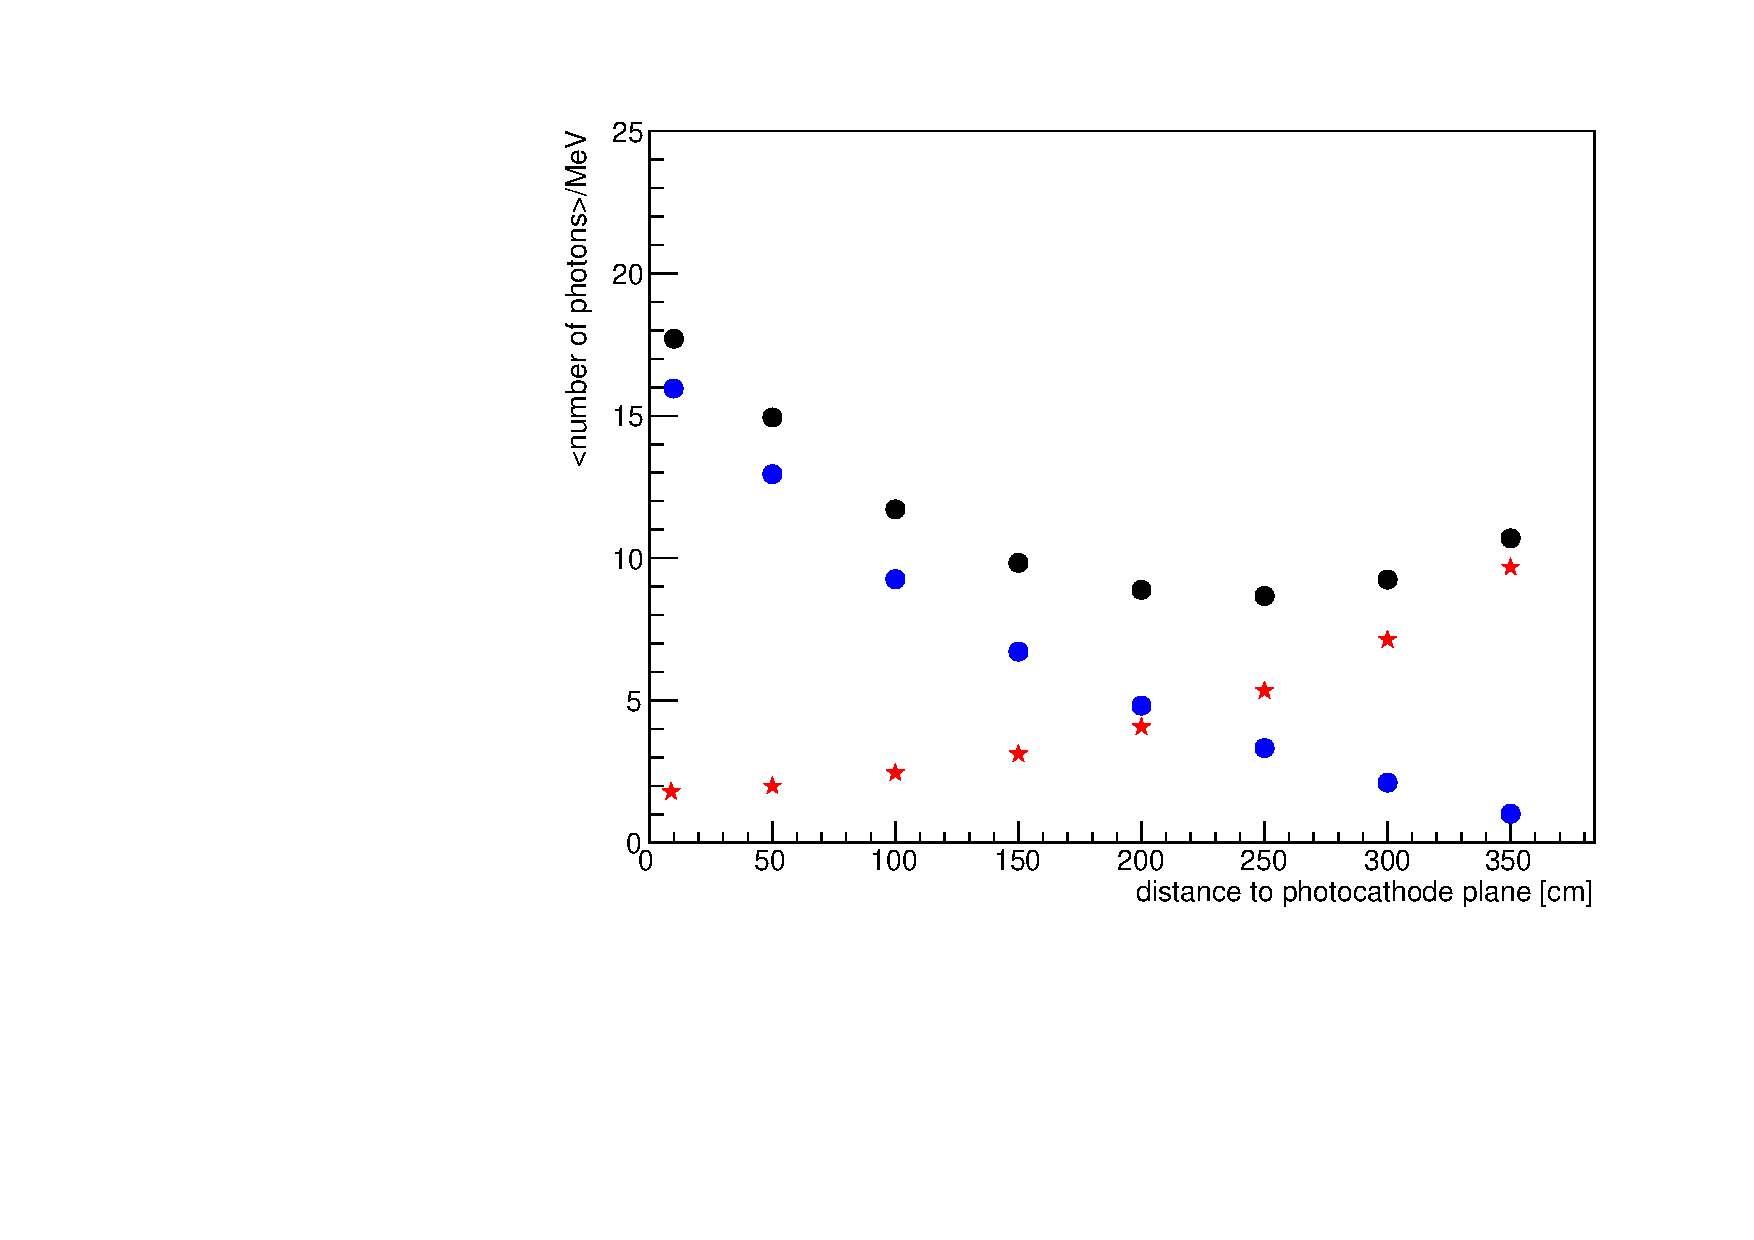
\includegraphics[width=0.6\columnwidth]{pds-ly_with_foils.pdf}
\end{dunefigure}

%<< Start: Andrzej Szelc 14/02/2018 <<<<<<<<<<<<<.

%% Remove Anode Plane Light Concentrators due to lack of development 4/9/18
%\subsubsection{Anode Plane Light Concentrators}
%\label{sec:fdsp-pd-assy-lc}
%\todo{\color{blue} Content: Cavanna}
	
%In the current baseline layout, the photosensitive area of the \dword{pds} is limited to about 12.5\% of the total area of the anode plane so a large fraction of the scintillation light produced in an event passes through the plane region undetected. 
%Increase in light collection, both for the \dword{vuv} and the reflected visible component (if the \dword{tpb}-coated foils at the cathode plane is adopted), can be achieved by implementing large area reflective surfaces at the anode plane in the large open areas between \dword{pd} bars inside the \dword{apa} frames. These would act as light concentrators toward the smaller photosensitive surfaces.  

%A conceptual solution, illustrated in Figure~\ref{fig:aplc}, is suggested by the widely used implementation of Winston Cones for enhancing light collection in large volume liquid detectors. 
%The \dword{pd} bar geometry of the photosensitive area inside the thin \dword{apa} frames and the related mechanical constraints impose rather severe limitations on the design - cone depth and entrance$/$exit apertures ratio - of the light concentrating surfaces. It is also the case that installation of the reflective surfaces inside the \dword{apa} frame would necessarily be made before wire winding. 
%Ongoing studies are expected to demonstrate the feasibility of the solution and move the conceptual scheme into a technical design. MC simulations will determine the efficiency of the light concentrator. 
%\fixme{it is difficult to picture what is intended without a figure}

%%\begin{dunefigure}[Anode Plane Light Concentrators schematic.]{fig:aplc}
%{Anode Plane Light Concentrators schematic. Note: just a placeholder for now.}
%\vspace{7cm}
%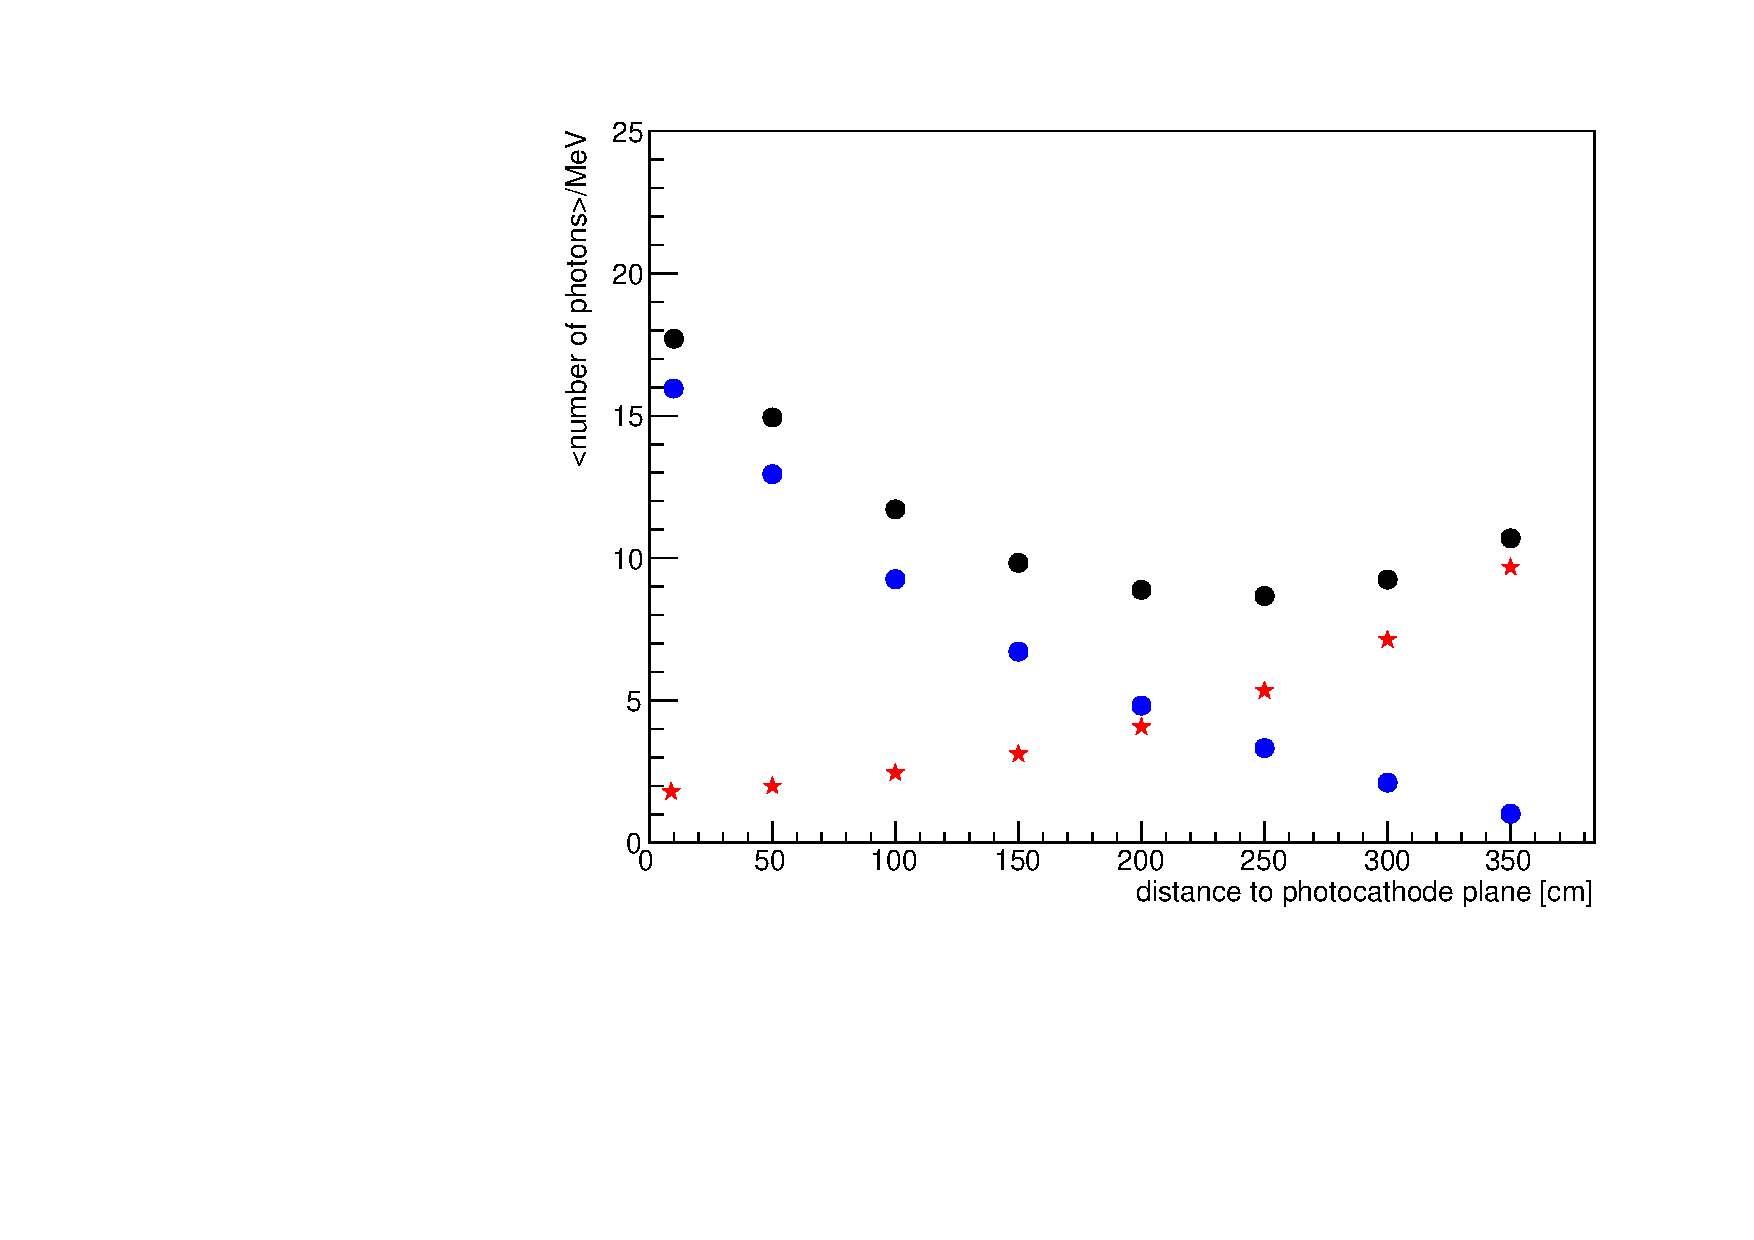
\includegraphics[width=0.5\columnwidth]{pds-ly_with_foils.pdf}
%\end{dunefigure}

%% Remove Anode Plane Light Concentrators due to lack of development 4/9/18

%% Move the Wavelength-Shifter Coated \dword{sipm} to the introduction of the ARAPUCA.
%\subsubsection{Wavelength-Shifter Coated \dword{sipm}} 
%The photon detectors described in the preceding section represent the results of a long process of optimization of the initial concepts developed years ago. A balance between the cost of the readout electronics (channel count), and the cost and performance of the \dword{sipm}'s was achieved with realistic designs of the photon detectors offering the detection efficiency in the range $\sim$ 0.5 to 2\%.
 
%Significant advances in the technology of the SPM's have been accomplished during this time: the photosensors dark count, after-pulsing and cross-talk rates have been lowered by almost an order of magnitude, whereas the production costs have been dropping significantly in response to the increasing range of applications.  The recent studies and tests demonstrate that the improved quality of the photodetectors is permitting much higher degree of ganging (passive or active), thus significantly lowering the "per \dword{sipm}" readout costs. These technological trends are likely to continue, thus allowing for a possible alternative concepts of the photon detectors, even within the geometrical and cost confines of the baseline detectors.

%One of the possible different concepts of the \dword{pd} includes a long printed circuit board with the overall dimensions identical to the light guide bars or ARAPUCA but with a simpler construction involving only \dwords{sipm} distributed over the board surface. The \dwords{sipm} can be coated with  appropriate wavelength-shifter (\dword{tpb} or MSB) or a foil with the wavelength-shifter in front of the \dword{sipm} can be used to convert the \dword{vuv} 128 nm Argon light to the blue light at the maximum detection efficiency of the \dword{sipm}. The overall detection efficiency of such a ``detector element" could be of the order of 25-30\%, depending on the pixel size and the fill-factor of the \dword{sipm}.

%A photon detector involving the \dwords{sipm} only would offer a major simplification of the construction and integration efforts. Its overall performance can be reliably estimated and it is proportional to the total area of the bar covered with the \dwords{sipm}. The performance of the baseline Photon Detectors can be achieved with 2-4\% of the area covered with the \dwords{sipm}. Taking 1800 cm$^2$ as a bar surface this coverage can be accomplished with 100-200 \dwords{sipm} of the standard 6x6 mm form factor. With 12-fold passive ganging, successfully demonstrated in recent tests, such a solution would require 8-16 readout channels per bar. The multiplexing level is limited by the noise of the readout electronics. Significantly higher degree of multiplexing can be achieved by use of larger pixel (e.g. 75x75 micron$^2$) \dwords{sipm} and/or possible cold active ganging circuitry. Though not yet developed, such a detector concept appears very flexible and it would allows for future optimization in response to the expected technological advances with no or minimal impact on the rest of the DUNE detector.  Since large-area solid state sensor technology will be beneficial also to the ARAPUCA design the \dword{pd} consortium will stay in close contact with photosensor manufacturers and monitor developments carefully in the coming years.




%%%%SILICON PHOTOSENSORS %%%%%%%%%%%%%%%%%%%%%%%%%%%%%%%%%%%%%%%%%%%%%%%%%%%

\subsection{Silicon Photosensors}
\label{sec:fdsp-pd-ps}
%\todo{\color{blue} Content: Zutshi}

The \dword{spmod} \dword{pds} uses a multi-step approach to scintillation light detection with final stage of conversion into electrical charge performed by silicon photomultipliers (\dword{sipm}). Robust photon detection efficiency, low operating voltages, small size and ruggedness make their use attractive in the \single design where the photon detectors must be accommodated inside the \dword{apa} frames. 
As implemented in \dword{pdsp}, there are twelve \num{6}$\times$\num{6}\si{mm$^2$} \dwords{sipm} per bar and 6-12 per ARAPUCA box.
With this configuration, a \SI{10}{kt} \dword{spmod} with \num{150} \dwords{apa}, each with \num{10} \dword{pd} modules, would contain \num{18000}-\num{36000} (single or double-ended readout) \dwords{sipm} for the light guide designs and 10-20 times more for the higher granularity ARAPUCA design. This corresponds to approximately \num{1}-\SI{13}{m$^2$} of active \dword{sipm} surface area.

In the following we summarize the most salient guiding principles and requirements for this \dword{sipm}-based photodetection system.

\begin{itemize}

\item  The full suite of \dword{sipm} requirements (number of devices, spectral sensitivity, dynamic range, triggering, 
zero-suppression threshold etc.) is determined by the physics goals and the photon collection implementation.  As discussed in Section~\ref{sec:fdsp-pd-intro},  the requirements for \dword{snb} neutrinos are not yet fully established however, 
R\&D carried out to date indicates that devices from several vendors have the 
performance characteristics close to that needed for the \dword{pds} (see Table~\ref{tab:photosensors}). 
Nearly one thousand of several types of these devices are used in the \dword{pdsp} \dword{pd}\footnote{\dword{pdsp} \dword{pds} uses 516 sensL MicroFC-60035C-SMT, 288 Hamamatsu MPPC 13360-6050CQ-SMD with cryogenic packaging, 180 Hamamatsu MPPC 13360-6050VE.}, which will provide an excellent test bed for evaluating and monitoring \dword{sipm}
performance in a realistic environment over a period of months.

\item A key requirement is to ensure the mechanical and electrical integrity of these devices in a cryogenic environment. However, currently, catalogue devices for most vendors are certified for operation only down to -40$^\circ$C. It is essential to be in close communication with  vendors in the design, fabrication and \dword{sipm} packaging certification stages to ensure that the device will be robust and reliable for long-term operation in a cryogenic environment. 
Two sources have expressed interest to engage with the consortium in this fashion with the goal of having the vendor warranty the product for our application: Hamamatsu Photonics K.K., a large well-known commercial vendor in Japan and Fondazione Bruno Kessler (FBK) in Italy, an experienced developer of solid state photosensors that typically licenses its technology and which is partnering with the DarkSide collaboration to develop a devices with very similar requirements as DUNE. 
Contact with other vendors and experiments using this technology in a similar environment is being pursued. 

\item Comparative performance evaluation of promising \dword{sipm} candidates from
multiple vendors will need to be carried out in parallel over the next year. This evaluation will need to
address inherent device characteristics (gain, dark rate, x-talk, after-pulsing etc), which are common to all three photon collector options, along with ganging performance, form factor, spectral response, and mechanical mounting options that may have different optimization for the two light guide design and ARAPUCA.
Experience acquired from \dword{pdsp} construction and operation will inform QA/QC plans for the full detector, which will need to be delineated in detail.

\item The optimal \dword{sipm} may depend on the photon collector option selected.  All 
options currently being considered involve shifting the \SI{127}{nm} \lar scintillation light to 
longer wavelengths, but each may present a different  spectral distribution to the \dword{sipm}. 
In this case, final selection of the \dword{sipm} might be delayed to allow an optimal match to the photon collector. 
However, we would not expect this fine-tuning to be more than a 15-20\% effect, so it is not a driving factor.

\item For the light guide photon collector designs, the \dword{sipm} packaging should allow for tileable arrays to be constructed to facilitate high packing efficiency across the end of the bars and efficient space utilization inside the \dword{apa} frame. 

\item Current candidate \dwords{sipm} have an area of less than \SI{1}{cm$^2$}, a much finer granularity than needed. In addition, the cold feedthrough size and space in the \dwords{apa} for cable runs limits  the number of \dword{pd} signal and power cables. These constraints, and other considerations, imply that the signal output of \dwords{sipm} must be electrically ganged. The degree of ganging depends on the photon collectors technology and currently ranges from six \dwords{sipm} for the light guides to \num{48} or more for the ARAPUCA modules. Whether simple passive-ganging (wiring the outputs together) will suffice or if active-ganging (with active components) is under investigation as a joint responsibility of the photon sensor and electronics working groups (see Section~\ref{sec:fdsp-pd-elec-intro} for more details).

\item The terminal capacitance of the sensors strongly affects the signal-to-noise when devices are ganged in parallel and so is a factor in \dword{sipm} selection, and may ultimately determine the maximum number of individual sensors that can be ganged this way. 

%\item To maintain signal quality, the \dword{sipm} signal path must be separate from the TPC readout. This implies that there must be cables dedicated to bringing the power in and taking the analog or digitized signals from the \dword{pds} out of the cryostat. So, in addition to the desire for channel count reduction to reduce readout electronics cost, feedthrough cable space limitations will also imply some level of electrical ganging of the \dword{sipm} signals inside the \lar volume. Investigation of this issue is being pursued in collaboration with the \dword{apa} consortium by the respective interface groups.
\end{itemize}

\begin{dunetable}[Candidate photosensors characteristics.]
{p{0.18\textwidth}p{0.18\textwidth}p{0.18\textwidth}p{0.18\textwidth}p{0.18\textwidth}}
{tab:photosensors}
{Candidate Photosensors Characteristics.}
	                         &Hamamatsu                           & sensL                                 & KETEK                       & Advansid                    \\ \toprowrule
Series part \#            & S13360                                 & DS-MicroC                         & PM33                          & NUV-\dwords{sipm}                \\ \colhline
Vbr range                 & 48 V to 58 V                           & 24.2 V to 24.7 V                & 27.5 V                         & 24 V to 28 V               \\ \colhline
Vop range                 & Vbr + 3 V                               & Vbr +1 V to +3 V               & Vbr+2V to +5 V           & Vbr +2 V to +6 V         \\ \colhline
Temp. dependence   & 54 mV/K                                & 21.5 mV/K                         & 22 mV/K                      & 26 mV/K                      \\ \colhline
Gain                           & $1.7 \times 10^6$                  & $3 \times 10^6$                & $1.74 \times 10^6$      & $3.6 \times 10^6$       \\ \colhline
Pixel size                   & 50 $\mu$m                            & 10 $\mu$m to 50 $\mu$m & 15 $\mu$m to 25 $\mu$m     & 40 $\mu$m       \\ \colhline
Sizes                          & 2x2 mm                                 & 1x1                                    & 3x3                               & 4x4                             \\ \colhline
                                  & 3x3 mm                                 & 3x3                                    &                                      & 3x3                             \\ \colhline
                                  & 6x6 mm                                 & 6x6                                    &                                      &                                    \\ \colhline
Wavelength                & 320 to 900 nm                       & 300 to 950 nm                  & 300 to 950 nm              & 350 to 900 nm            \\ \colhline
PDE peak wavelength  & 450 nm                               & 420 nm                             & 430 nm                         & 420 nm                       \\ \colhline
PDE @ peak              & 40\%                                     & 24\% to 41\%                    & 41\% at Vov=5 V          & 43\%                           \\ \colhline
DCR @0.5PE             & 2 to 6 MHz                            & 0.3 kHz to 1.2 MHz          & 100 kHz  at Vovr=5 V   & 100 kHz/mm$^2$       \\ \colhline
Crosstalk                    &< 3\%					& 7\%                                  & 15\%                             &  < 4\% (correlated noise) \\ \colhline
Afterpulsing                &                                               & 0.20\%                             & \textless 1\%                 & \textless4\%               \\ \colhline
Terminal capacitance & 1300 pF                                 & 3400 pF                           & 750 pF                          &800 pF                         \\ \colhline
Lab experience          & Good experiences from Mu2e and ARAPUCA & Crack at LN2 temps. after specifications change&         &     \\         
\end{dunetable}

% From Kurt Francis 4/13/18
% Hamamatsu crosstalk is < 3%; for  Advansid/FBK they report the combined afterpulsing and delayed crosstalk as �correlated noise� which is < 4%.

%%%%%%%%%%%%%%%%%%%%%%%%%%
%The planned photodetector is a \dword{sipm}, model 
%SensL C-Series 6~mm$^2$
%(MicroFB-60035-SMT). % device. 
%This model of \dword{sipm} has a detection efficiency of
%41\%; the quoted detection efficiency incorporates Quantum Efficiency (QE) and 
%the effective area
%  coverage accounting for dead space between pixels.   At \lar temperature (89~K) the dark rate is of order 10~Hz
%(0.5 p.e. threshold), and  after-pulsing has not been observed. An on-going testing program is in place to ensure 
%that the \dwords{sipm} can reliably survive the stresses associated with 
%any thermal cycling in \lar and long-term operation at \lar temperature.

%All photodetectors %for \dword{pdsp} 
%are subjected to testing to determine
 %forward and reverse bias I-V curves,
 %breakdown voltage, dark current and dark count rate, photodetector gain, crosstalk estimation, response, and bias dependence of parameters.
 
%All \dwords{sipm} 
%Each \dword{sipm} is tested before mounting on the readout boards to determine
%if the part meets the specifications in a warm test.  After mounting to
%the readout board all items are tested both warm and cold (cyrogenic 
%temperature) to determine the operating characteristics.

%In addition to these tests, the photodetectors are tested for their
%response to light signals from an LED of appropriate wavelength.
%These tests will be sensitive enough to determine if one of the three \dword{sipm}
%elements operating in parallel is not functioning.


%%%%ELECTRONICS %%%%%%%%%%%%%%%%%%%%%%%%%%%%%%%%%%%%%%%%%%%%%%%%%%%

\subsection{Electronics}
\label{sec:fdsp-pd-pde}
%\metainfo{\color{red}\bf  Content: (3 pages) - Djurcic/Franchi/Moreno}
%rjw 4/10/18 \fixme{electronics conveners please check for accuracy} -- no responses

\subsubsection{Introduction}
\label{sec:fdsp-pd-elec-intro}

%DWW 16mar18 start %%%%%%

% I am re-doing all this…

%The photon-detector design requires the readout system to collect and process electric signal from photo-sensors in \lar, 
%to provide interface with trigger and timing systems to support data reduction and classification, and to enable data transfer 
%to an offline storage for physics analysis.

%The photon-readout is required to enable the detector measurement of the time-zero of non-beam events with deposited 
%energy above \SI{200}{MeV}. This capability will also enhance beam physics, by recording interaction time of events within 
%beam spill to help separate against potential cosmic background interactions. In addition, any consideration of pulse-shape 
%discrimination will require capability to record both prompt and delayed components of scintillation light, latter one consisted mostly 
%from single photo-electrons at readout end. Photon-detector collects a limited amount of light, so it could be beneficial to 
%collect the light from both excited states. Therefore, important physics questions that may affect the design of the electronics 
%readout system include understanding of required time resolution for the photon readout system, and clarification whether 
%the system needs to efficiently collect single photo-electron signals. 

%Simplification in the readout scheme and a cost reduction will come from reading arrays of \dwords{sipm}, rather than individual 
%photo-sensors. To that end we desire a system where the single \dword{sipm} array reads a whole photodetector unit.
%Technical factors that affect performance of the system are type of the selected \dword{sipm} with characteristic capacitance, 
%number of \dwords{sipm} connected together with a choice of "ganging" scheme, to dictate signal to noise ratio and affect the system 
%performance and design considerations. Selection of the ganging option will include passive or active solutions, where the active 
%circuitry may require cold components such as an amplifier in \lar volume. Design options with active cold components will need 
%to address issues of power dissipation and potential risks of single-point failures of multi-channel devices inside the cryostat.
%In the case of passive ganging, analog signals are transmitted outside of the cryostat for processing and digitalization. 

%In general arrival time and total charge are the parameters to be obtained from a detector. Extraction of these parameters 
%is possible using analog or digital systems. Charge preamplifier is usually connected to the output of the detector to integrate 
%current producing a charge proportional output. In the case of digital systems an amplifier is needed to adjust the detector output signal 
%level to the input of an Analog to Digital Converter.  In both systems, performance parameters related  to sampling rate, number of bits, 
%power requirements, signal to noise ratio, and interface requirements should be evaluated to arrive to selected solution.  
%Pulse shapes can be fully analyzed to improve detection of a new physics but it will have an important impact on the digitalization %frequency.

The \dword{pd} design requires the readout system to collect and process electrical signals from photosensors reading out the light collector bars, 
to provide interface with trigger and timing systems to support data reduction and classification, and to enable data transfer 
to offline storage for physics analysis.

%The readout system must enable the measurement of the time-zero of non-beam events with deposited energy above \SI{200}{MeV}. 
The readout system must enable the measurement of the t$_0$ of non-beam events with deposited energy above \SI{10}{MeV}. 
This capability will also enhance beam physics, by recording interaction time of events within 
beam spill to help separate against potential cosmic background interactions. Two main methods of data collection are currently considered:  self-triggered integrated charge readout and wave form digitization.  Charge integration appears to be a likely candidate at this point in our development, as it offers the potential for a simpler, commercially available charge integration circuit and perhaps a smaller, less-expensive cable plant to read it out.  Physics simulation studies are currently underway to determine if pulse-shape discrimination will be required, which would provide the capability to record both prompt and delayed components of scintillation light (characteristic times of \SI{6}{ns} and \SI{1.3}{$\mu$s}), the latter consisting mostly of single photoelectrons and thus place stringent requirements on signal-to-noise performance. The photon detector collects a limited amount of light, so it could be beneficial to collect the light from both excited states. 
%Therefore, important physics questions that may affect the design of the electronics readout system include understanding of required time resolution for the photon readout system, and clarification whether the system needs to efficiently collect single photoelectron signals. 
Since this requirement has not yet been established the option is kept open in the electronics design.

%Simplification in the readout scheme and a cost reduction can also be realized by reading arrays of \dwords{sipm}, rather than individual photosensors.
All photon collector options will require some level of electrical ganging of the \dwords{sipm}, either passive direct connection of the \dword{sipm} outputs or active (cold signal summing and possibly amplification).  To that end we desire a system where the ganging is maximized to minimize the electronics channel count while maintaining adequate redundancy and granularity, as well as readout system performance.  This represents a significant interface between the electronics, photosensor and light collector designs, and will be a main focus of our development and optimization work up to the \dword{tdr}.

Technical factors that affect performance of the ganging system are the characteristic capacitance of the \dword{sipm} 
and the number of \dwords{sipm} connected together, which together dictate the signal to noise ratio and affect the system 
performance and design considerations. Selection of the ganging option will include passive or active solutions, where the active 
circuitry may require cold components such as an amplifier in the \lar volume. Design options with active cold components will need 
to address issues of power dissipation and potential risks of single-point failures of multi-channel devices inside the cryostat.
In the case of passive ganging, analog signals are transmitted outside of the cryostat for processing and digitalization. 
Successful demonstrations of passive ganging at \lar temperatures have been made for groups of four and twelve 6x6 mm Micro-FC-60035C-SMT C series, and groups of 2, 4, 8, and 12  Hamamatsu MPPCs (S13360-6050PE) at  \num{25}$^\circ$C, - \num{70}$^\circ$C and \SI{77}{K}. Active ganging has been demonstrated for an array of 12 sensL \num{4}$\times$\num{4} arrays of \SI{3}{mm}$\times$\SI{3}{mm} sensL C-series \dwords{sipm} (48 in all) and  72 \dwords{sipm} mounted in a hybrid combination of passive and active ganging using \SI{6}{mm}$\times$\SI{6}{mm} MPPCs with a low noise operational amplifier--this design combines 12 active branches into the op-amp, where each branch has 6 MPPCs in a parallel passive-ganging configuration.
%\fixme{9 apr18 decide which Gustavo figures to use }

Typically, arrival time and total charge are the key parameters to be obtained from a detector. Extraction of these parameters 
is possible using analog or digital systems. Charge preamplifiers will be connected to the output of the detector to integrate 
current producing a charge proportional output. In the case of digital systems an amplifier is needed to adjust the detector output signal 
level to the input of an Analog to Digital Converter.  In both systems, performance parameters related  to sampling rate, number of bits, 
power requirements, signal to noise ratio, and interface requirements should be evaluated to arrive to selected solution.  
Pulse shapes can be fully analyzed to improve detection of a new physics but it will have an important impact on the digitalization frequency.

%DWW 16mar18 end %%%%%%
%\subsubsection{Photosensor Ganging}
%\label{sec:ganging}
%\fixme{9 apr18 New text from Gustavo - add some preamble text and clean up}
%R\&D on cold electronics and sensor arrays
%Under LDRD L2017.028 (P.I. Gustavo Cancelo) the \dword{pd} R\&D collaboration has developed and characterized several configurations of cold electronics and \dwords{sipm} as follow:
%\begin{itemize}
%\item A 48 \dword{sipm} summing board for SENSL 4x4 arrays. This is an active ganging board of 48 3mm x 3mm \dwords{sipm} from SenSL C series. This detector has been fully characterized and tested at \dword{tallbo} with an alpha source (Am241) in March 2017. For the \dword{tallbo} test the \dword{sipm} arrays were coated with \SI{100}{$\mu$g/cm$^2$} of \dword{tpb} and showed an efficiency of 13\%.
%\item A 12 SENSL (6x6 mm C series) summing board that was used by the IU group in their light bars during the \dword{tallbo} run of Oct-Nov 2017.
%\item We have tested Hamamatsu MPPCs (S13360-6050PE) at 25C, -70C and 77K. A passive ganging of 2, 4, 8 and 12 MPPCs were characterized and showed single PE separation.
%\item A passive gang of 4 SENSL (6x6 mm C series) for ARAPUCAs during the \dword{tallbo} run of Oct-Nov 2017.
%\item A passive gang of 6 and 12 MPPCs for ARAPUCA \dword{pdsp} design
%\item A 72 combination of passive and active ganging using 6mm x 6mm MPPCs with a lower noise OP Amp. This design combines 12 active branches into the low noise OpAmp. Each branch has 6 MPPCs in parallel passive configuration.
%\end{itemize}

%\fixme{9 apr18 decide which figures to use }

\subsubsection{ProtoDUNE-SP Electronics}

% For the bar-style photon-detectors the solution with three \dword{sipm} ganged together, being read-out through the single readout channels has been implemented. 

A dedicated photon-detector readout system, presented schematically  in Figure~\ref{fig:fig-pds-readout}(left), was developed for \dword{pdsp}, which will be operational in the second half of \num{2018}.  Twenty-four custom \dword{sipm} Signal Processor (SSP) units were produced to read out the 58 light guide and 2 ARAPUCAs photon collectors.  
An SSP contains of twelve readout channels packaged in  a self-contained 1U module; four SSPs are shown in Figure~\ref{fig:fig-pds-readout}(right).

A passive ganging scheme with three \dwords{sipm} ganged together was chosen for the light guides (4 SSP channels for each bar) and groups of twelve \dwords{sipm} are passively ganged for the two ARAPUCA modules (12 SSP channels per module).  The unamplified analog signals from the \dwords{sipm} are transmitted to outside the cryostat for processing and digitization over an approximately \SI{25}{m} cable to the SSP outside the cryostat. 
 Each channel receives the \dword{sipm} signal into a termination resistor that matches the characteristic impedance of the signal cable followed by a fully-differential voltage amplifier and a \num{14}-bit, \num{150}-MSPS analog-to-digital converter (ADC) that digitizes the \dword{sipm} signal waveforms. 
  
%\begin{dunefigure}[Block diagram of the \dword{pdsp} SSP module]{\dword{pd}_fig-e-3}{Block diagram of the \dword{pdsp} SSP module} 
%\includegraphics[width=\textwidth]{pds-\dword{pdsp}-SSP-block-diagram.png}
%\end{dunefigure}

 \begin{dunefigure}[\dword{pdsp} Photon Detector readout.]
 {fig:fig-pds-readout}
 {Block diagram of the \dword{pdsp} photon detector readout module (left). Photon detector readout system operational at \dword{pdsp} (right). }
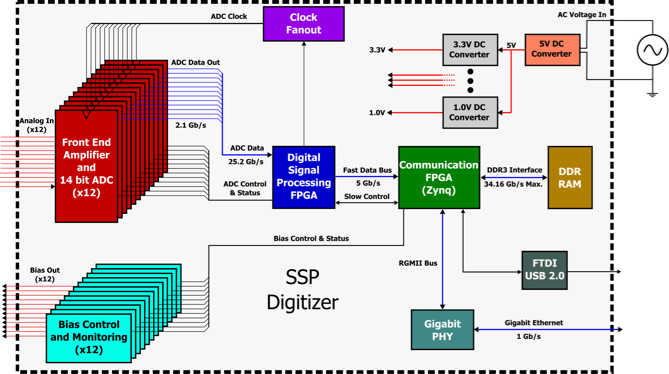
\includegraphics[angle=0,width=8.4cm,height=6cm]{pds-fig-e-3.png}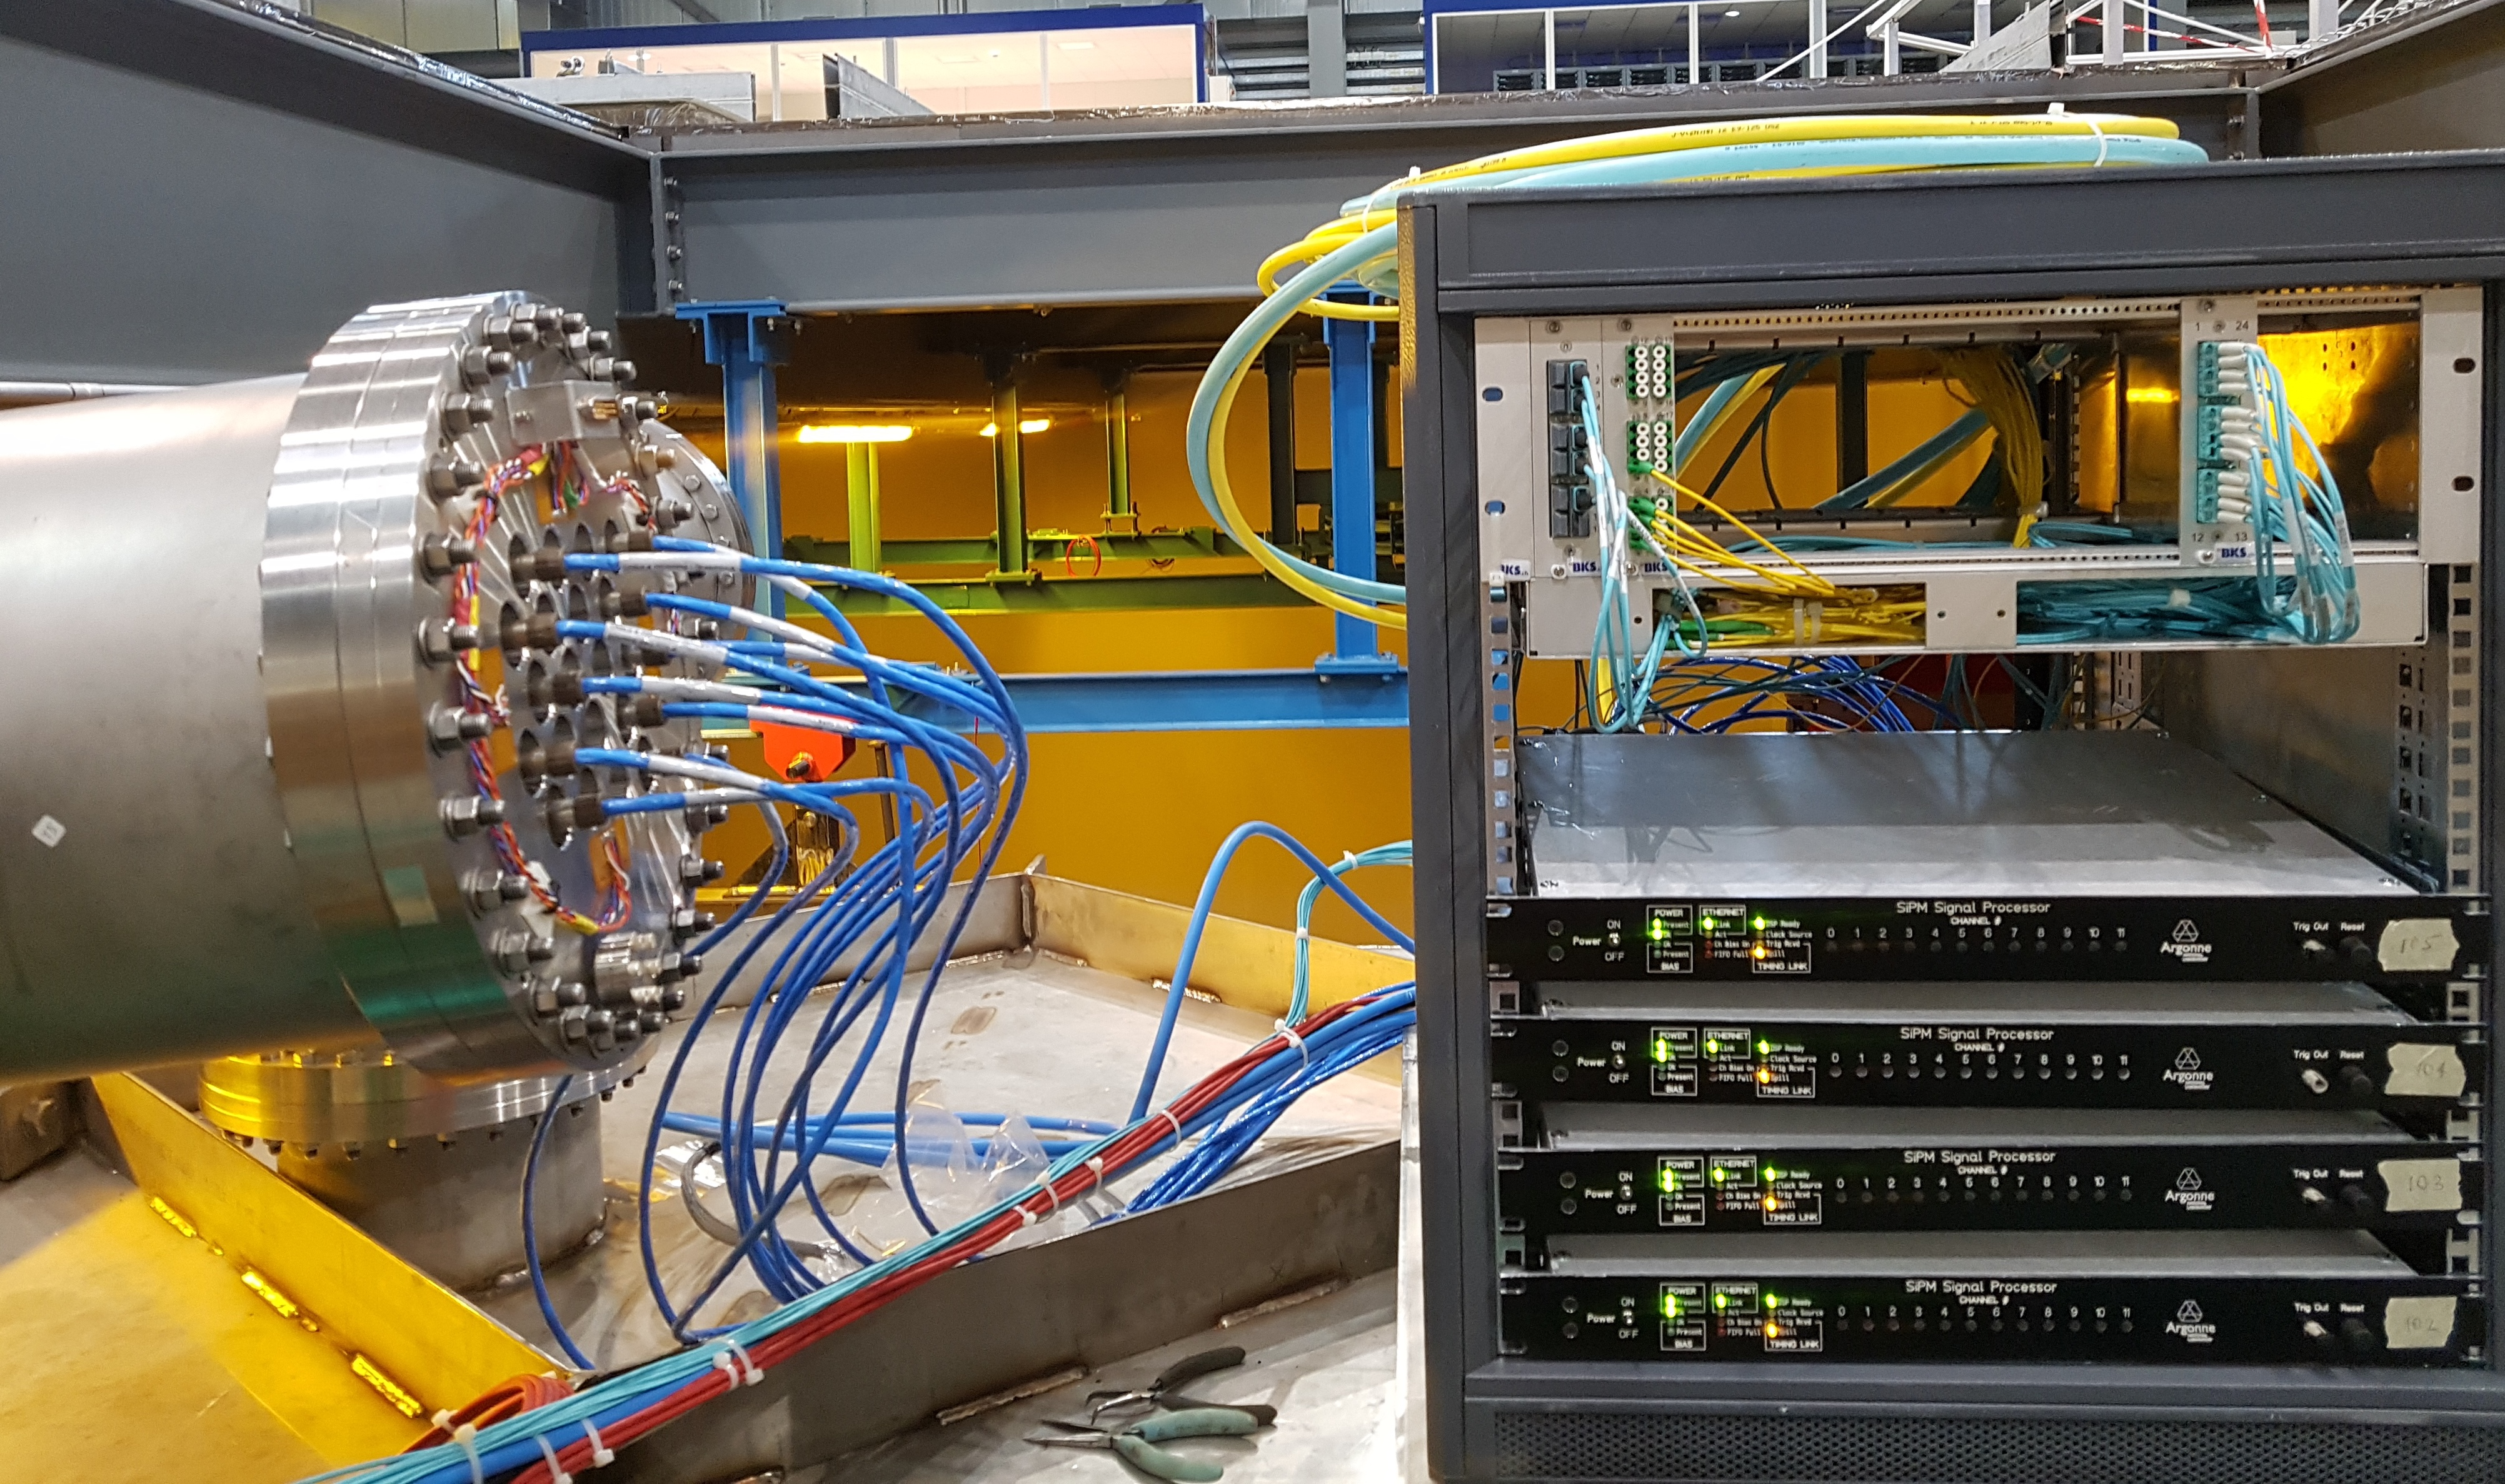
\includegraphics[angle=0,width=8.4cm,height=6cm]{pds-protodune_readout_coldbox.jpg}
\end{dunefigure}

In the standard mode of operation, the module performs waveform capture, using either an external or internal trigger. In the latter case the 
module self-triggers to capture only waveforms with an amplitude greater than a specified threshold. In \dword{pdsp} the photon readout 
is configured to read waveforms when triggered by a beam event, and/or to provide header information when self-triggered by cosmic muons.
The header portion summarizes pulse amplitude, integrated charge, and time-stamp information of events. The SSP for \dword{pdsp} uses \si{Gb} Ethernet 
communication implemented over an optical interface. The \SI{1}{Gb/s} Ethernet supports full TCP/IP protocol.  

The module includes a separate \num{12}-bit high-voltage DAC for each channel to provide bias to each \dword{sipm}\footnote{Currently there are two DAC options: one with a voltage range of \num{0}-\SI{30}{V}, used with the sensL \dwords{sipm} (17 of the 24 SSP units); and the other with a range \num{0}-\SI{60}{V} for use with the Hamamatsu MPPCs (7 of the 24 SSP units). }. The SSP provides a trigger output signal from internal discriminators in firmware based on programmable coincidence logic, with a standard ST fiber interface to the central trigger board (CTB).
Input signals are provided to CTB from the beam instrumentation, the SSPs, and the beam TOF system. The CTB receives timing information from 
the \dword{pdsp} timing system and the CTB trigger inputs are distributed to the experiment via the timing system.
To that end, the SSP implements the timing receiver/transmitter endpoint hardware to receive trigger inputs and clock signals from the timing system.


\subsubsection{Electronics Next Steps}

Although the requirements for the electronics system are not all fully established, it not expected that the system will require novel high-risk techniques and can be developed and fabricated well within the schedule for the \dword{pds}.
In the latter half of CY18, \dword{pdsp} test beam and cosmic-ray muon data analysis will provide evaluation of the readout system implemented in \dword{pdsp} and the \dword{pd} Photon Sensor and Simulation groups will provide essential guidance on optimization of performance and cost.

As identified in Section~\ref{sec:fdsp-pd-ps}, the most important near term R\&D program will be to optimize the ganging scheme including choice of \dword{sipm} and cable types. 
The first objective is to demonstrate that an ensemble of 48-72 Hamamatsu \SI{6}{mm}$\times$\SI{6}{mm} MPPCs can be summed into a single channel by a combination of passive and active ganging. This board will also measure the photoelectron collection efficiency when the \dwords{sipm} are coated with \dword{tpb} as a reference for ARAPUCA measurements with a similar ganging level (the summing  board is the same size as the \dword{pdsp} ARAPUCA backplane to facilitate the comparisons).
Charge processing requires a charge preamplifier ideally located within the cold environment, so the design must take into consideration the failure risks and the power dissipated into the environment.

The timing resolution, minimum threshold and dynamic range requirements for the system are dictated by the physics requirements. These are well known for the higher energy physics (>\SI{200}{MeV}) but, as noted elsewhere in this document, are still evolving for lower energy. Currently, 
a timing resolution of 1$\mu$s is called for and the sampling rate and number of sample bits is estimated based on this. For this task 
some digital process such as a sample interpolation may be proposed, enhancing the recorded raw sample time precision.
The light sensitivity and the dynamic range requirement will determine the number of bits and the sample rate required by either waveform or charge collection methods. In both cases, the signal to noise ratio and the power consumption must be estimated.  
With this data from \dword{pdsp} and the ganging studies, the choice between waveform readout and integrated charge readout will be made taking into account DAQ  readout and trigger requirements. 


%From Gustavo 10apr18
%The objective is to demonstrate that 72 MPPCs can be summed up in a single channel by a combination of passive and active ganging.
%Other steps to be covered by this design:
%Measure the PE collection efficiency covering the MPPCs with \dword{tpb} and measuring in \lar with a radio source.
%Measure the effective area of an ARAPUCA as a function of the number of MPPCs placed on the board. For this test the board becomes the backplane of an ARAPUCA. The size of the board is compatible with the size of the ARAPUCA used in \dword{tallbo} in 2017. Filters are available.




